\section{Introduction}
Here we learn about major non-hexapod arthropod lineages---\textbf{Chelicerata} (spiders, mites, scorpions, and their relatives), \textbf{Myriapoda} (centipedes, millipedes, and their relatives), and some non-hexapod \textbf{Pancrustacea} (pillbugs, brine shrimp, and their relatives)---including their natural histories and hypotheses of their evolutionary history. We'll also look at the likely sister to Arthropoda: \textbf{Onychophora} (velvet worms).

You should have a firm grasp of arthropod anatomy now. Before we start, revisit our discussion of the phenotypes that make an organism an arthropod. Now consider their diversity relative to other metazoans: vertebrates, annelids, nematodes, \textit{etc}. What phenotypes would you consider \latinword{key innovations} for Arthropoda? Why is Arthropoda orders of magnitude more diverse than its sister lineage? As you examine the specimens in the hands-on portion of this unit think about how the traits you observe inform us of the evolutionary history of these organisms.

\section{Onychophora (velvet worms)}\index{Onychophora}
\noindent{}\textit{Diagnostic characters:} Segmented and relatively soft body, with a single pair of antennae and serially homologous legs. Legs unsegmented. Tagmata not obvious.\vspace{3mm}

\noindent{}\textit{Natural history:} Velvet worms are predators of other invertebrates, usually subduing prey with a glue-like mucous that is excreted with force from glands near the mouth. They are quite susceptible to desiccation and so are usually found in humid habitats. There are approximately 200 species, which can found throughout the Neotropics and in pockets throughout the rest of the world. There is a rich fossil record of onychophoran-like organisms (``Lobopodia'') from marine environments, but there are no extant marine species.\vspace{3mm}

\begin{theo}[Onychophora]
{}Can you see any shared, derived characters (figures \ref{fig:onych},\ref{fig:onychLeg}) between onychophorans and arthropods? What traits indicate that these creatures are  \textit{not} Arthropoda?
\end{theo}

\begin{figure}[ht!]
  \centering
    \includegraphics[width=0.85\textwidth]{nonhexapod/onychophora}
  \caption{Onychophora habitus \citep[][Fig. 81]{bhlitem40112britmus}}
  \label{fig:onych}
\end{figure}

\begin{figure}[ht!]
  \centering
    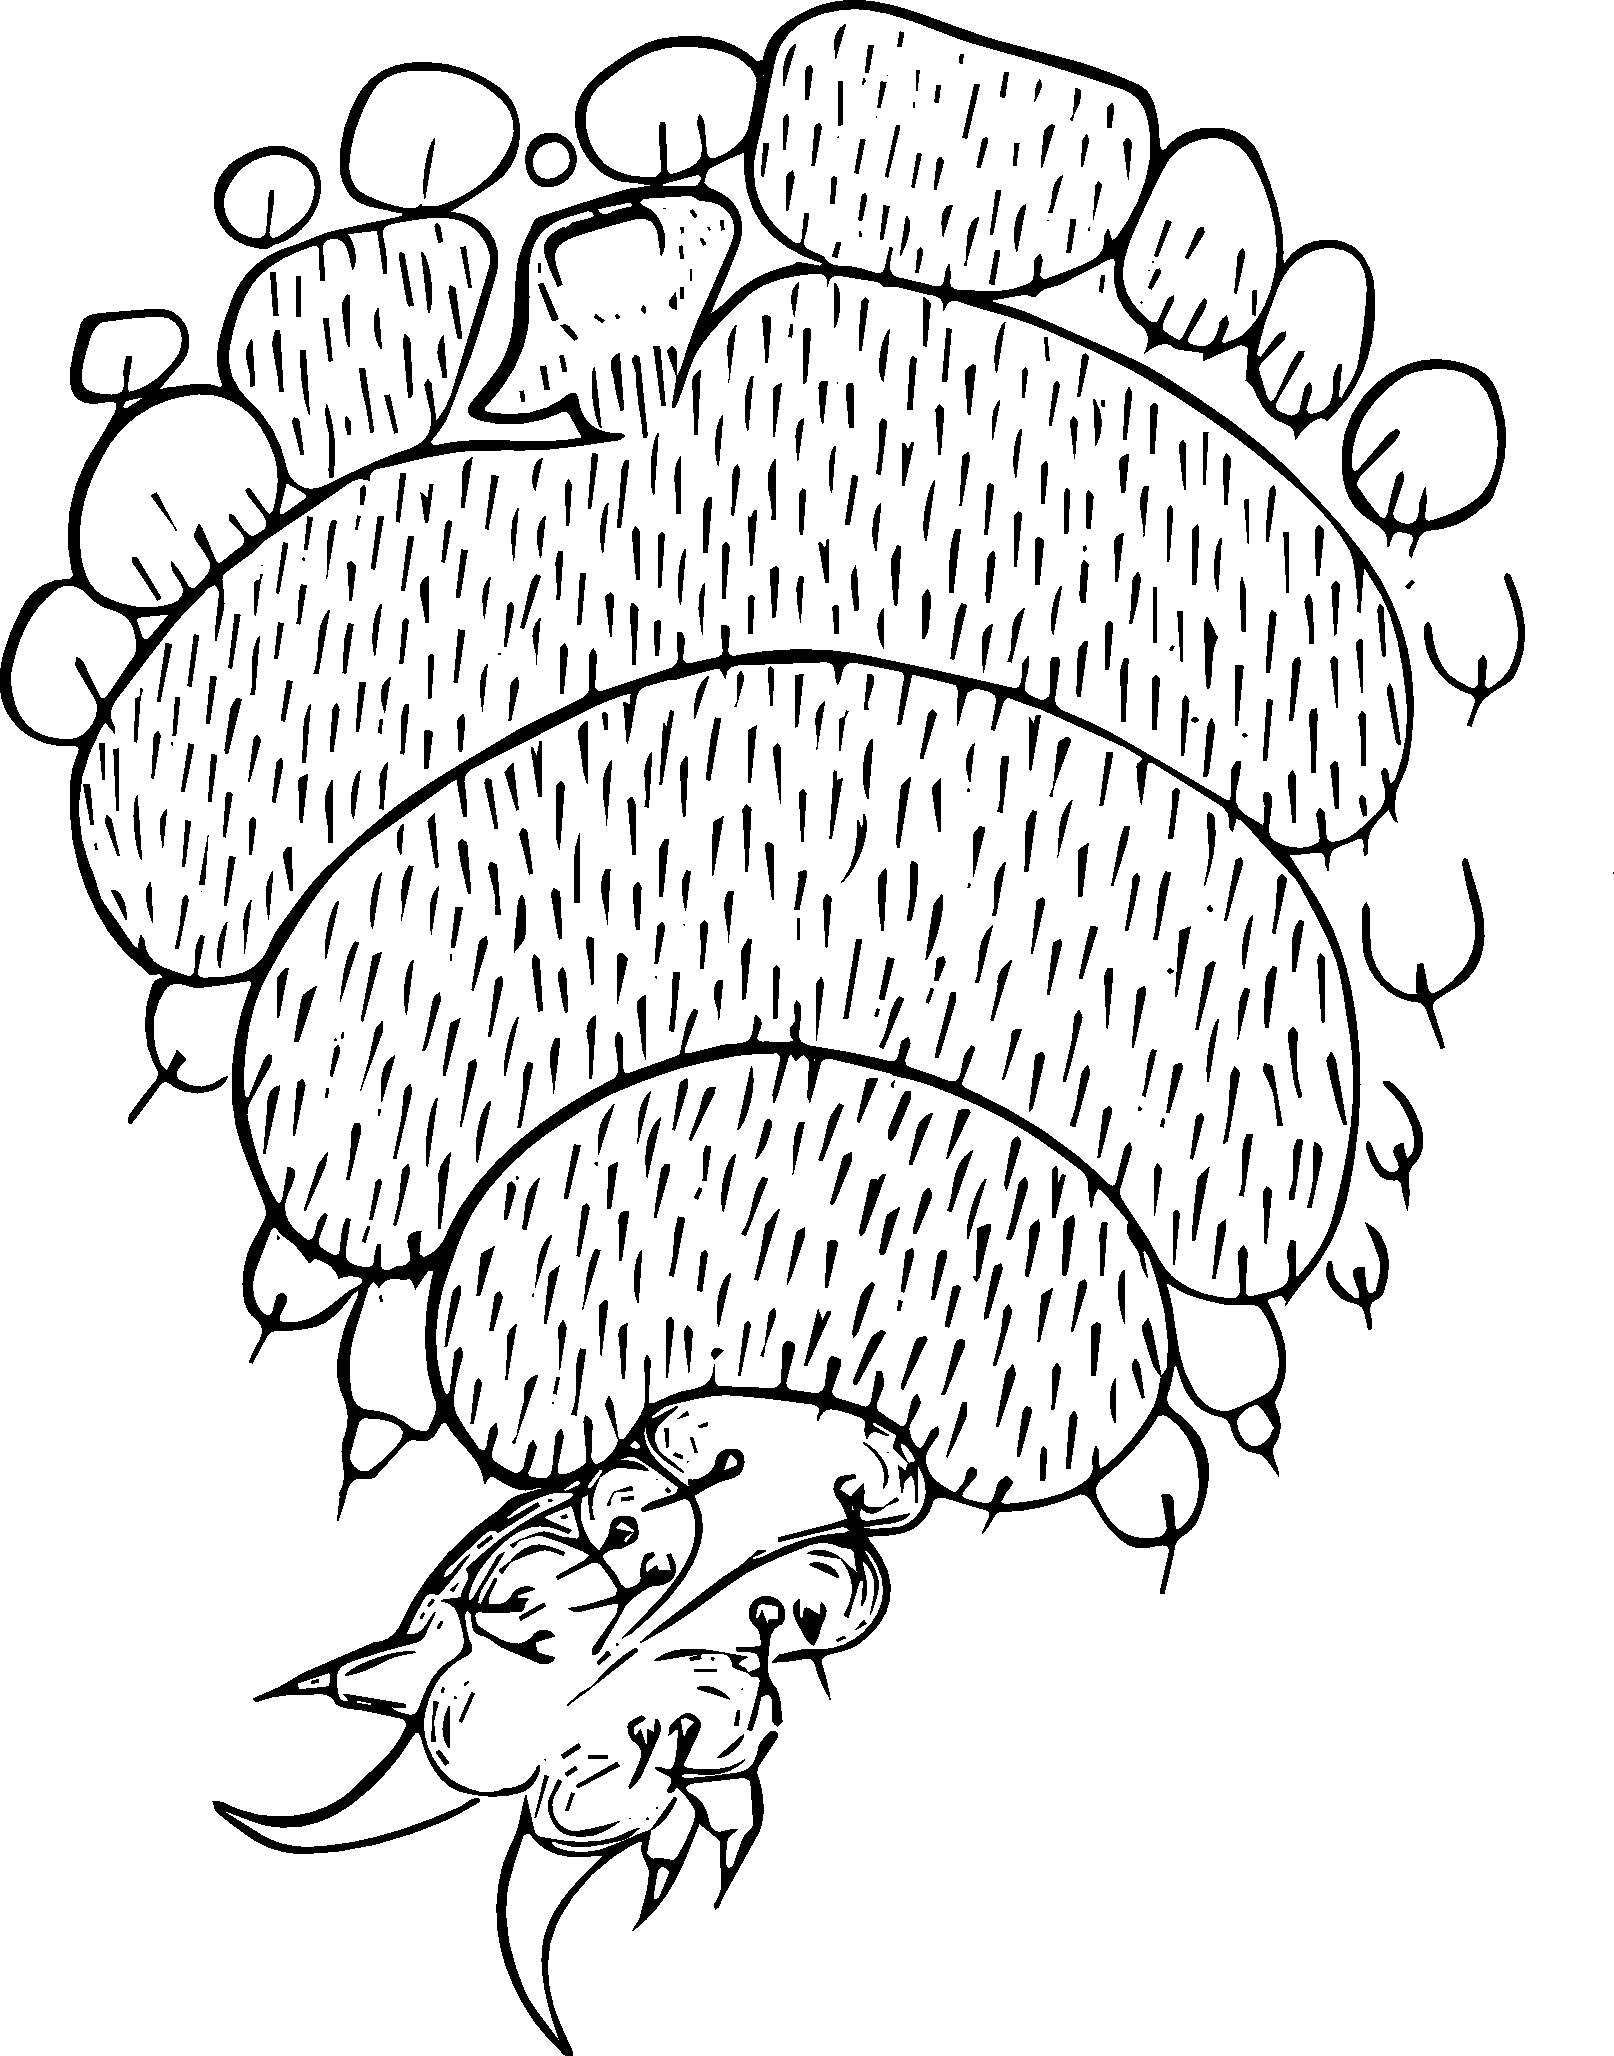
\includegraphics[width=0.22\textwidth]{nonhexapod/onychLeg}
  \caption{Onychophora leg \citep[][Fig. 6]{bhlpart201070OnychLeg}}
  \label{fig:onychLeg}
\end{figure}

\section{Chelicerata}\index{Chelicerata}
We are now looking at true arthropods, beginning with Chelicerata. Members of this lineage share the following characters: 
\begin{itemize}
\item antennae absent (though anteriormost pair of legs often antenniform)
\item 6 pairs of \latinword{uniramous} appendages: chelicerae (mouthparts) + pedipalps + 4 pairs of legs
\item 2 tagmata: \latinword{prosoma} (cephalothorax) and \latinword{opisthosoma} (abdomen)
\end{itemize}

\subsection{Xiphosura (horseshoe crabs)}\index{Xiphosura}
\noindent{}\textit{Diagnostic characters:} Prosoma covered by large carapace that has two compound eyes; appendages, including chelicerae, relatively uniform in morphology; book gill present; long spine (telson) present on posterior margin of opithosoma.\vspace{3mm}

\noindent{}\textit{Natural History:} Approximately four extant species known worldwide, all of which are marine. Their diet includes molluscs and other marine invertebrates, which they masticate with spines on the four anteriormost pairs of legs (gnathobase).\vspace{5mm}

\begin{theo}
{}Recent phylogenies reveal that Xiphosura is deeply embedded \textit{within} Arachnida \citep[\textit{e.g}.,][]{d13110568}. Do you see evidence that these arthropods are related to other Arachnida? What does this mean with respect to terrestrialization in Chelicerata?
\end{theo}

\begin{figure}[ht!]
  \centering
    \includegraphics[width=0.7\textwidth]{nonhexapod/xiphosura}
  \caption{Xiphosura \citep[][Fig. 9]{bhlitem21199comstock}}.
  \label{fig:xipho}
\end{figure}
%https://www.biodiversitylibrary.org/page/2822779

\noindent{}The most diverse group of chelicerates is \textbf{Arachnida}, which includes all the terrestrial species of Chelicerata. We will examine specimens of the arachnid taxa listed below. Can you see the diagnostic characters clearly? If you saw any of these specimens in a lab practical could you name it (with correct spelling), describe a diagnostic feature, and/or describe its natural history?

\subsection{Araneae (spiders)}\index{Araneae}
\noindent{}\textit{Diagnostic characters:} Chelicerae fang-like (figure \ref{fig:fang}); anteriormost pair of legs not antenniform; pedipalps not chelate, rarely stouter than legs; opisthosoma not obviously segmented (except rarely); opisthosoma attached to prosoma via narrow constriction (figure \ref{fig:spider}); spinnerets present posteroventrally on opisthosoma, but no tail-like structure (telson).\vspace{3mm}

\noindent{}\textit{Natural History:} Incredibly diverse taxon, with more than 50,000 described species found worldwide and in almost every habitat. These arthropods are well known for their use of silk to form webs, tunnels, ``parachutes'', and other contraptions. They are all predators, although some will supplement their diets with pollen or other plant products.\vspace{3mm}

\begin{theo}[Araneae]
{}Find three spiders that look very different from each other, \textit{e.g.}, a tarantula, a jumping spider, and an orb weaver or cellar spider. Examine and sketch their eye patterns. Are they different? Find three males of different species and examine and sketch their pedipalps. Can you homologize their parts?\vspace{3mm}

\noindent{}Compare the chelicerae of a tarantula and an orb weaver or jumping spider. See any differences? Now compare the ventral habitus of their opisthosomata.\vspace{3mm}

\noindent{}Why do spiders have a constricted ``waist'', a trait not generally seen in other chelicerates?
\end{theo}

\begin{figure}[ht!]
    \centering
    \begin{subfigure}[ht!]{0.2\textwidth}
        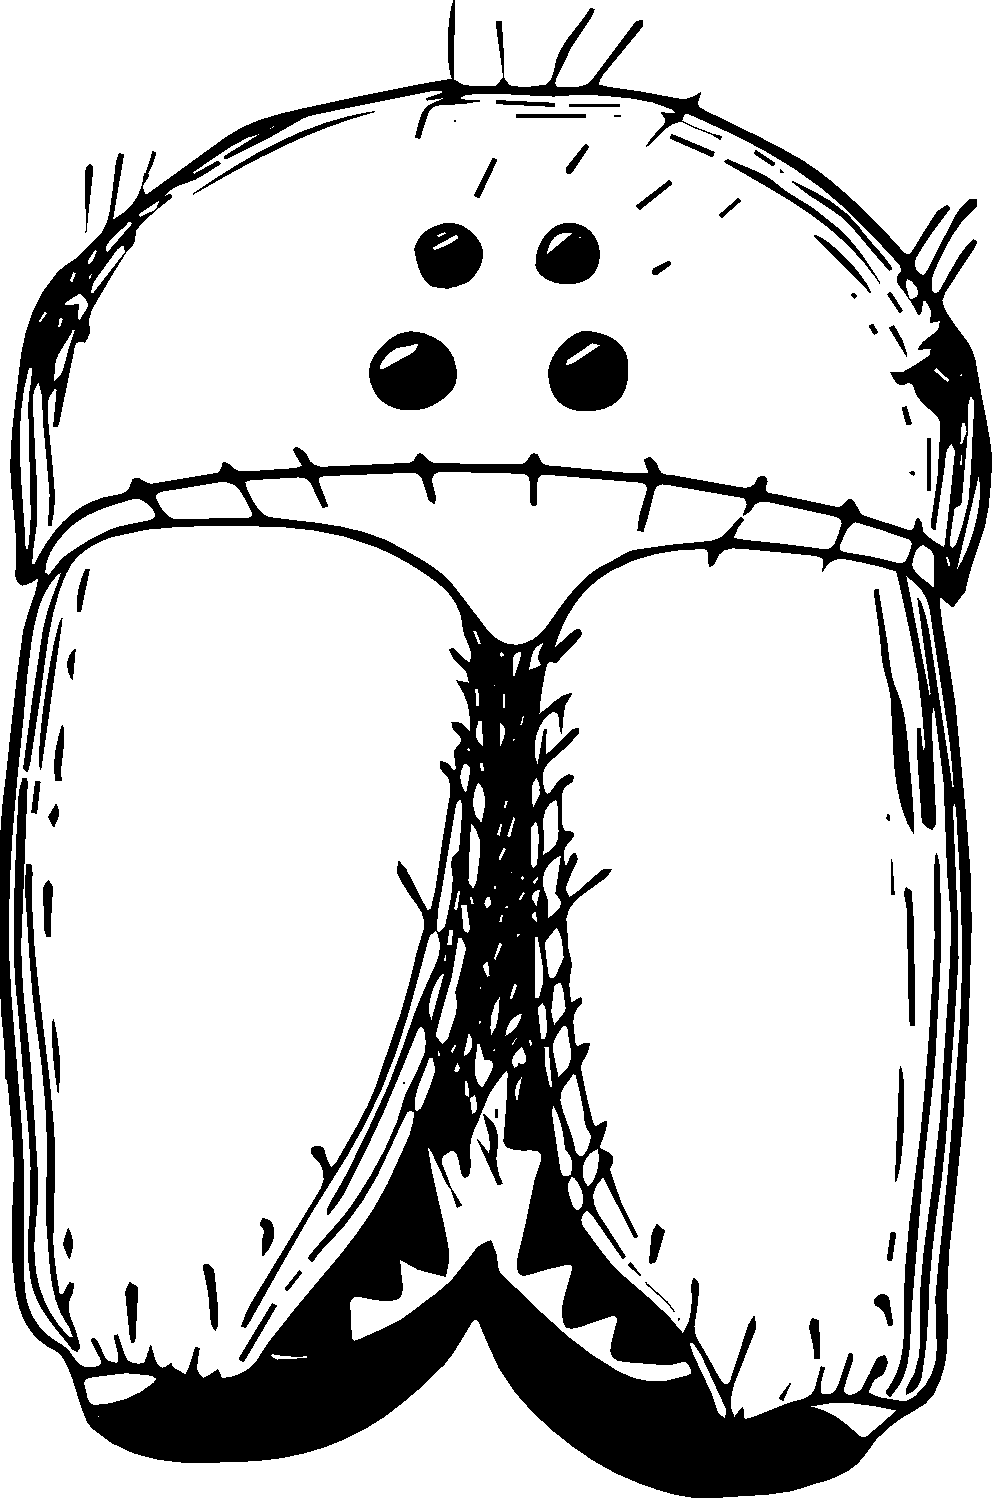
\includegraphics[width=\textwidth]{nonhexapod/spider78}
        \caption{}
        \label{fig:fang}
    \end{subfigure}
    \hfill
    \begin{subfigure}[ht!]{0.7\textwidth}
        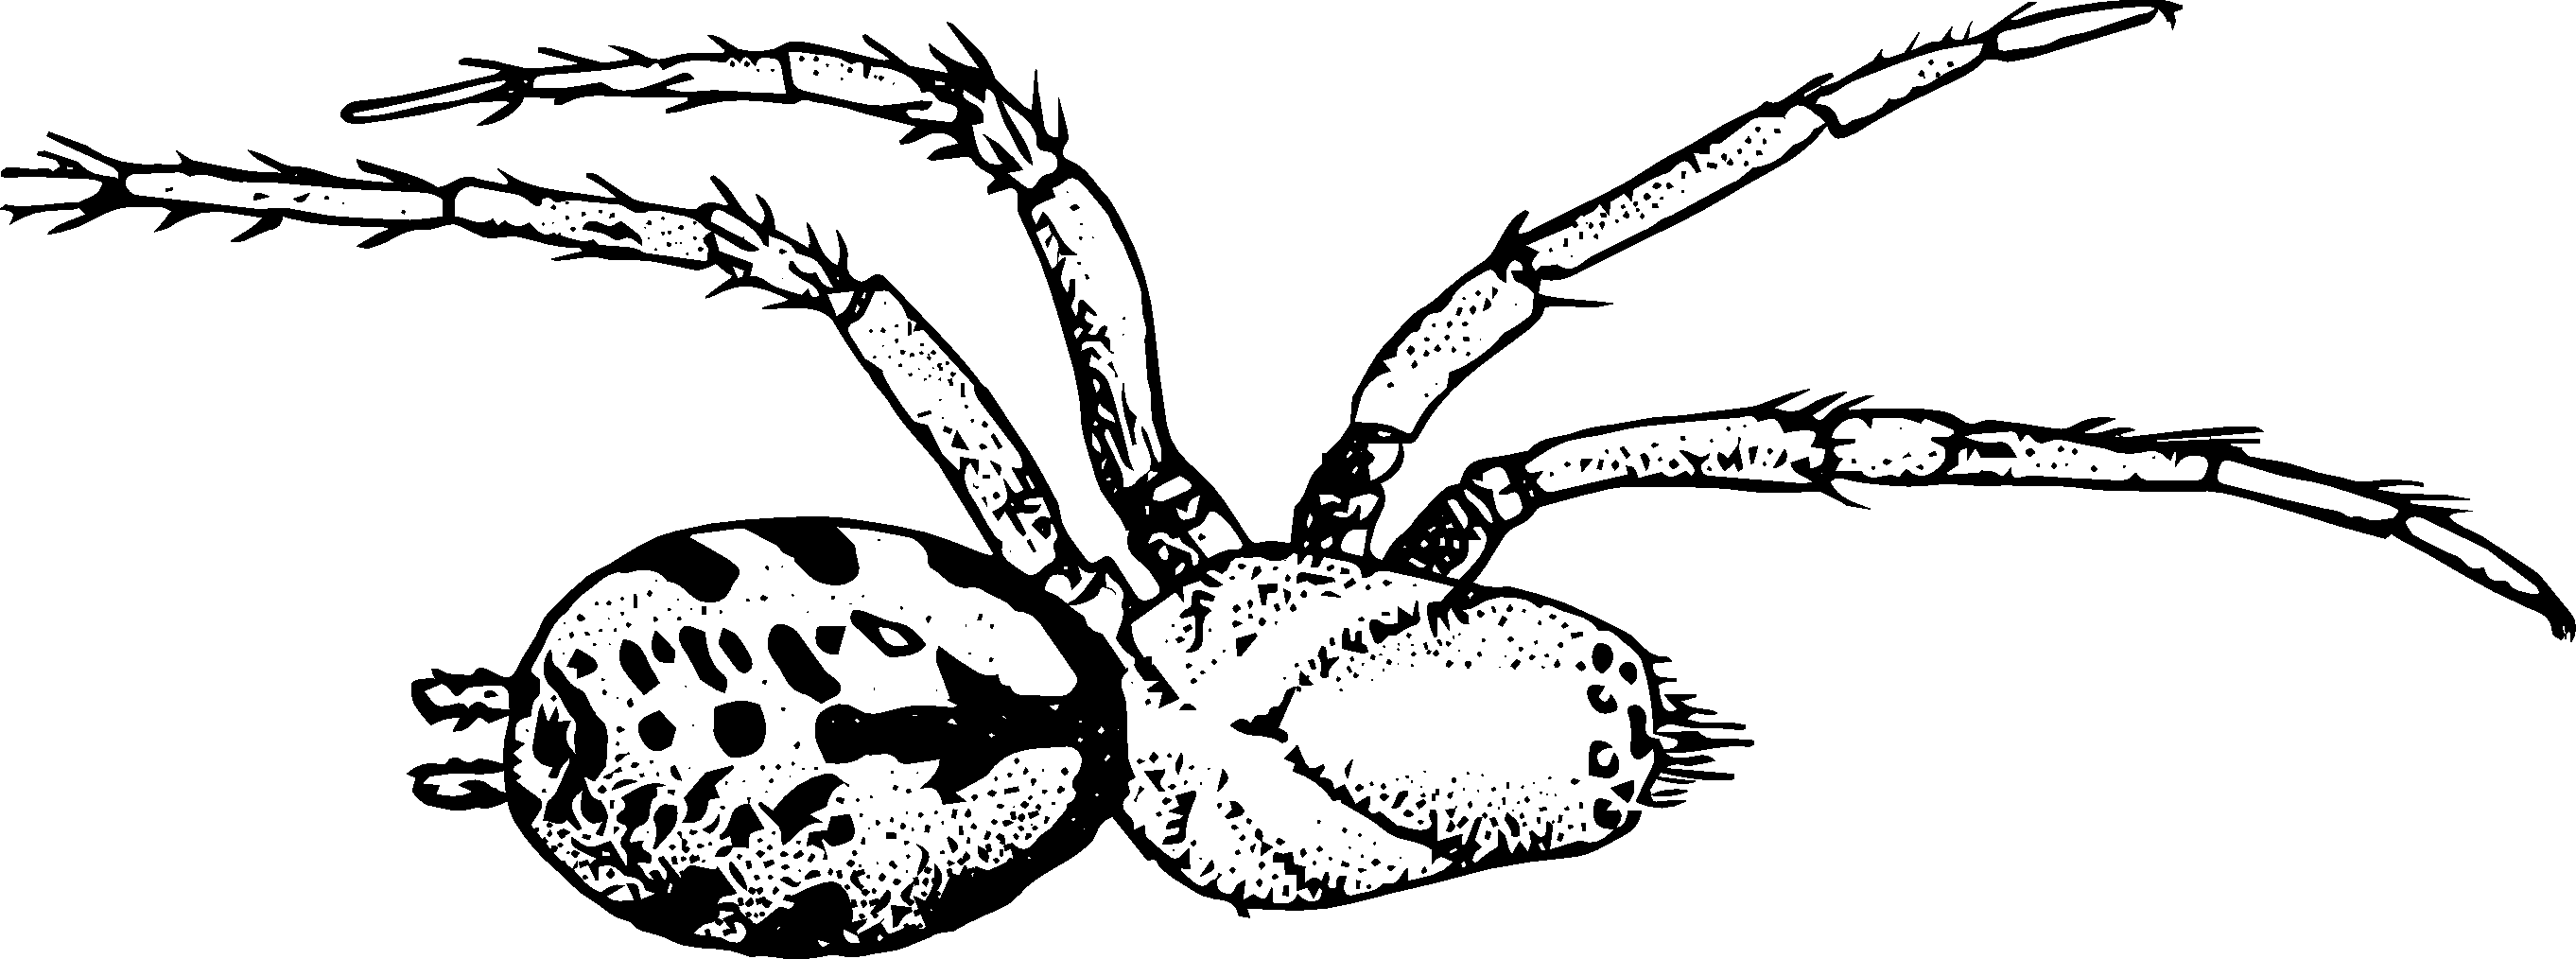
\includegraphics[width=\textwidth]{nonhexapod/spider314a}
        \caption{}
        \label{fig:spider}
    \end{subfigure}
    \caption{Spiders (Araneae). \textbf{(a)} Head in anterior view \citep[][Fig. 78]{bhlitem21199comstock}; \textbf{(b)} dorsal habitus \citep[][Fig. 314a]{bhlitem21199comstock}}\label{fig:spiders}
\end{figure}

\subsection{Acari (Acarina, mites, ticks)}\index{Acari}
\noindent{}\textit{Diagnostic characters:} Opisthosoma not segmented (See figure \ref{fig:mites}); opisthosoma broadly joined to prosoma, no tail-like structure (telson); young instars with 3 pairs of legs, adults with 4; pedipalps not chelate, not thicker than legs; mouthparts usually project anteriorly, chelicerae not chelate; usually very small (0.08--10 mm body length).\vspace{3mm}

\noindent{}\textit{Natural History:} Another incredibly diverse taxon, with more than 44,000 described species found worldwide. It is difficult to generalize their natural history, as there are species that feed as predators, herbivores, detritivores, fungivores, and parasites, and they live in just about every habitat imaginable. Recently people have started treating these arthropods as two superorders: Acariformes (mites, including eyelash mites and those that cause mange) and Parasitiformes (ticks and parasitic mites).\vspace{3mm}

\begin{theo}
{}Based on their mouthpart morphology, can you make \textit{any} generalization or predictions about mite feeding habits?
\end{theo}

\begin{figure}[ht!]
    \centering
    \begin{subfigure}[ht!]{0.4\textwidth}\reflectbox{
        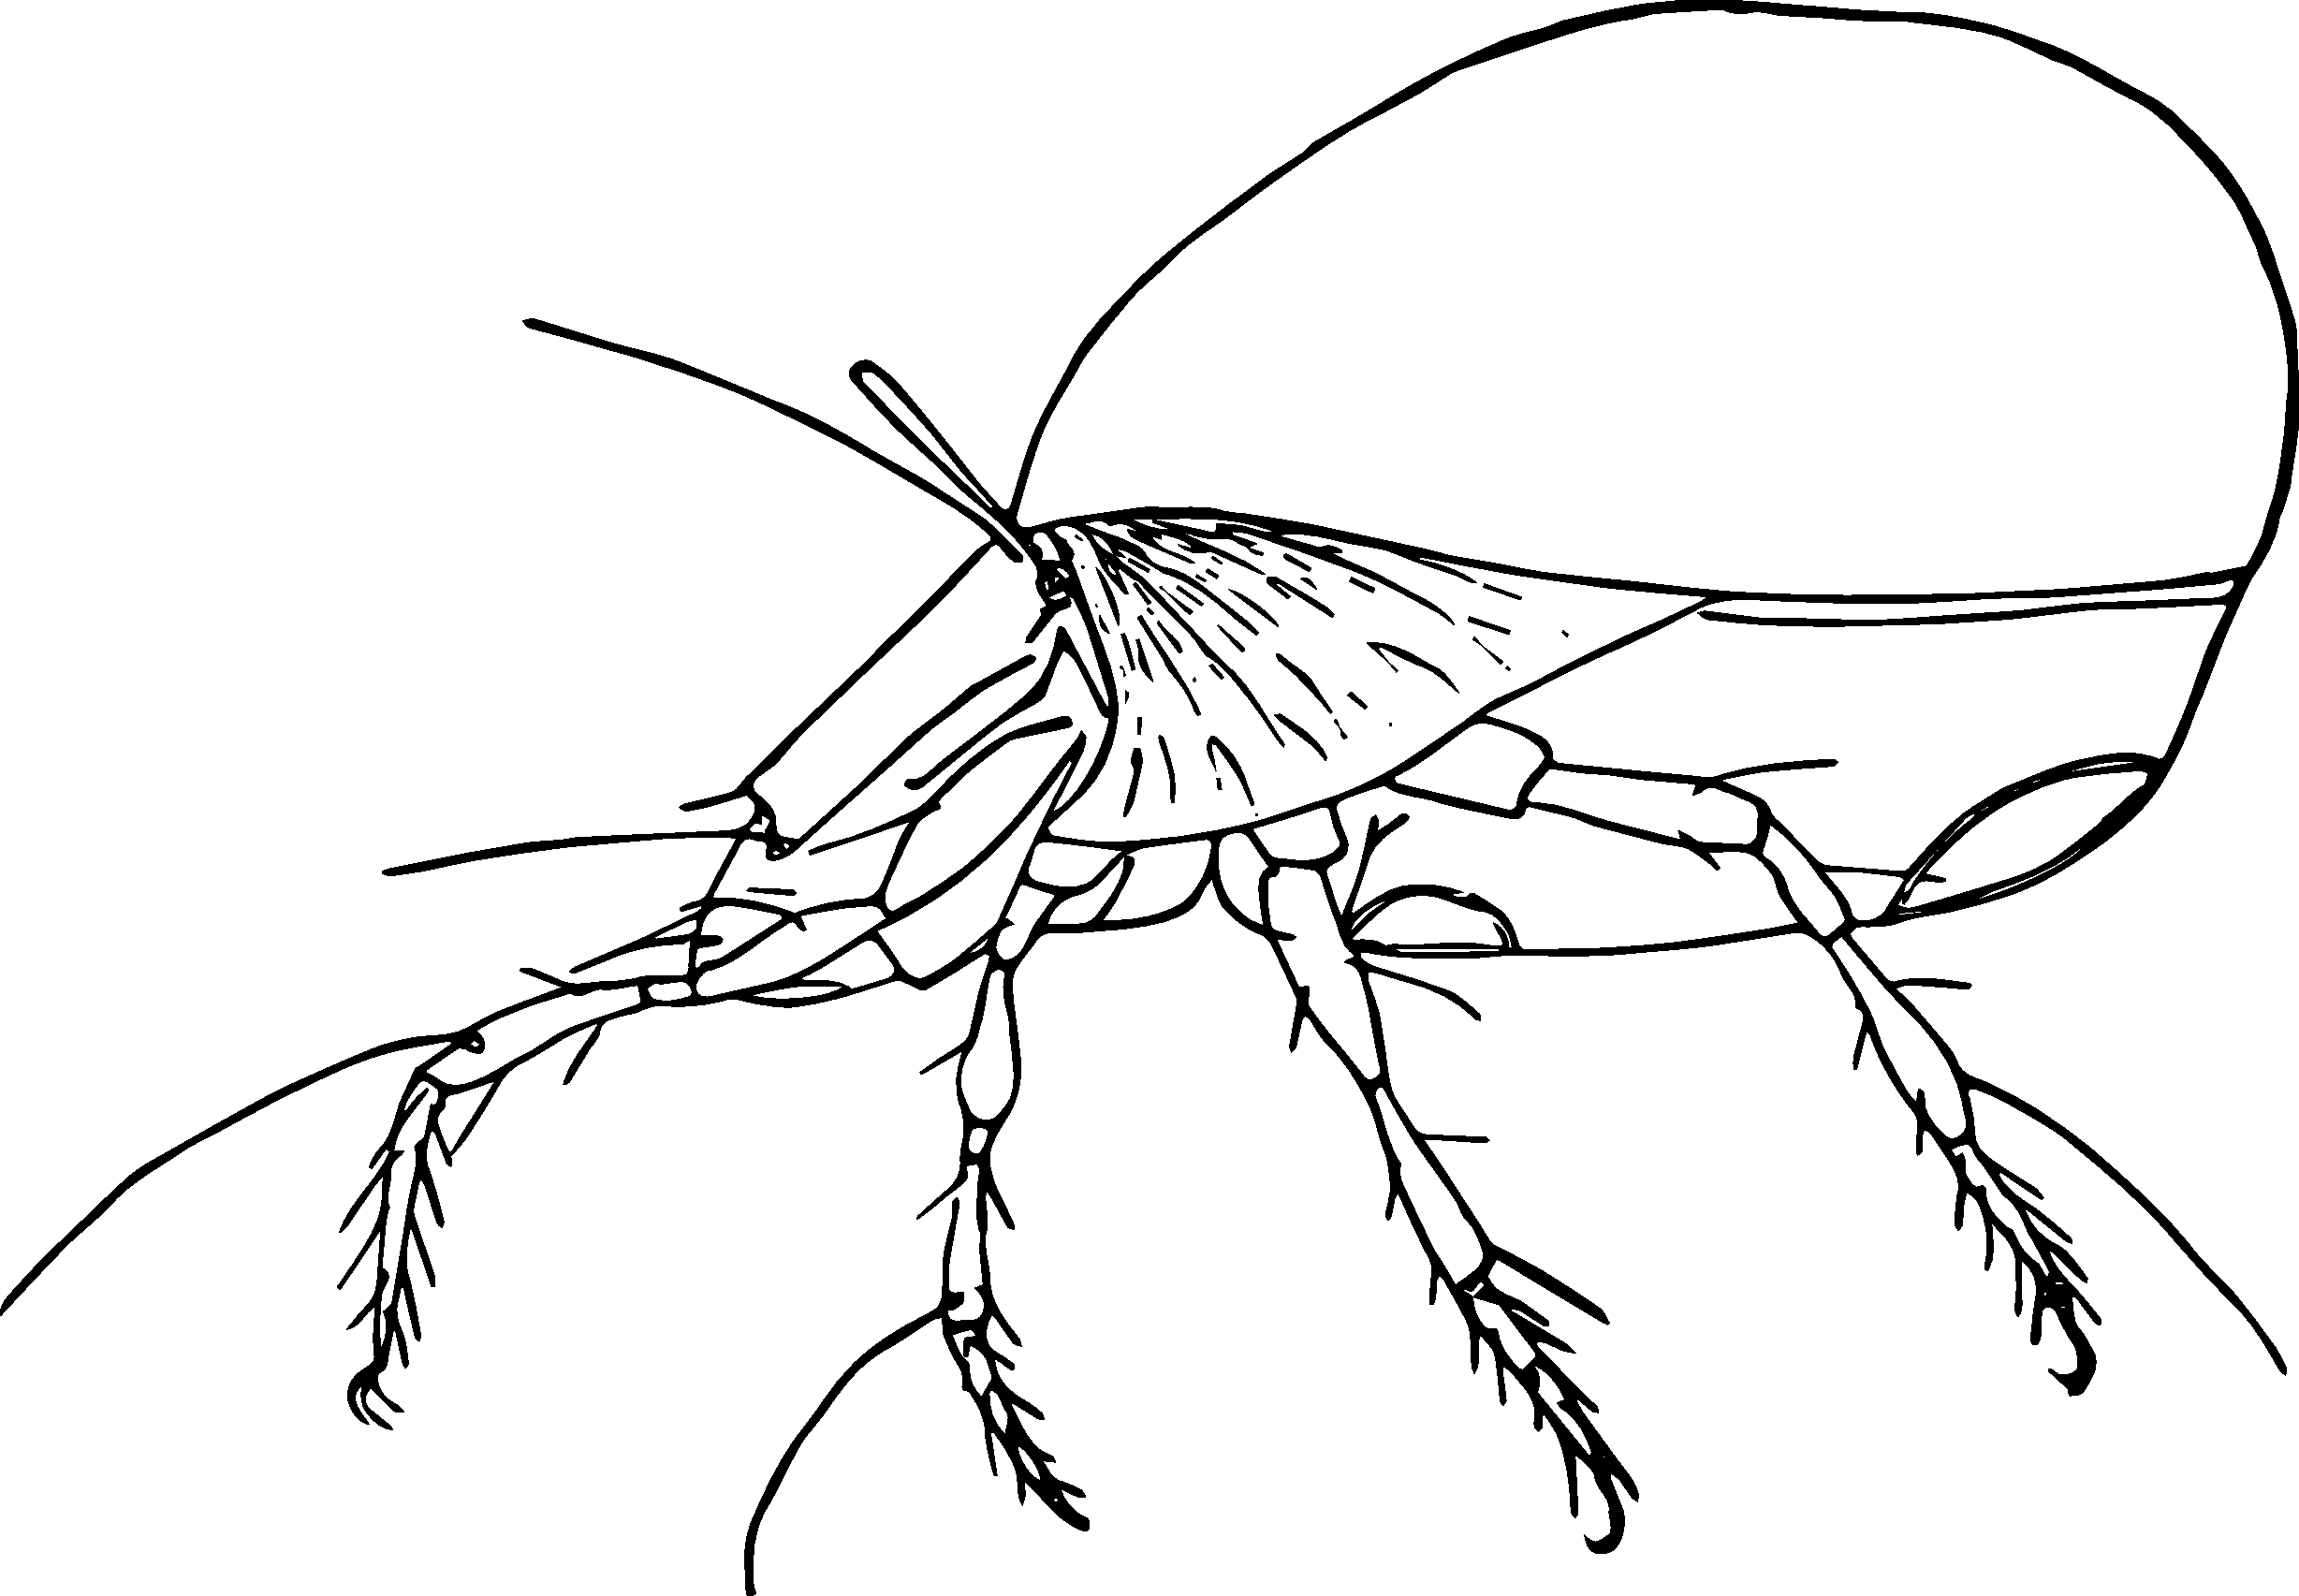
\includegraphics[width=\textwidth]{nonhexapod/oribatid}}
        \caption{}
        \label{fig:mite1}
    \end{subfigure}
    \hfill
    \begin{subfigure}[ht!]{0.45\textwidth}
        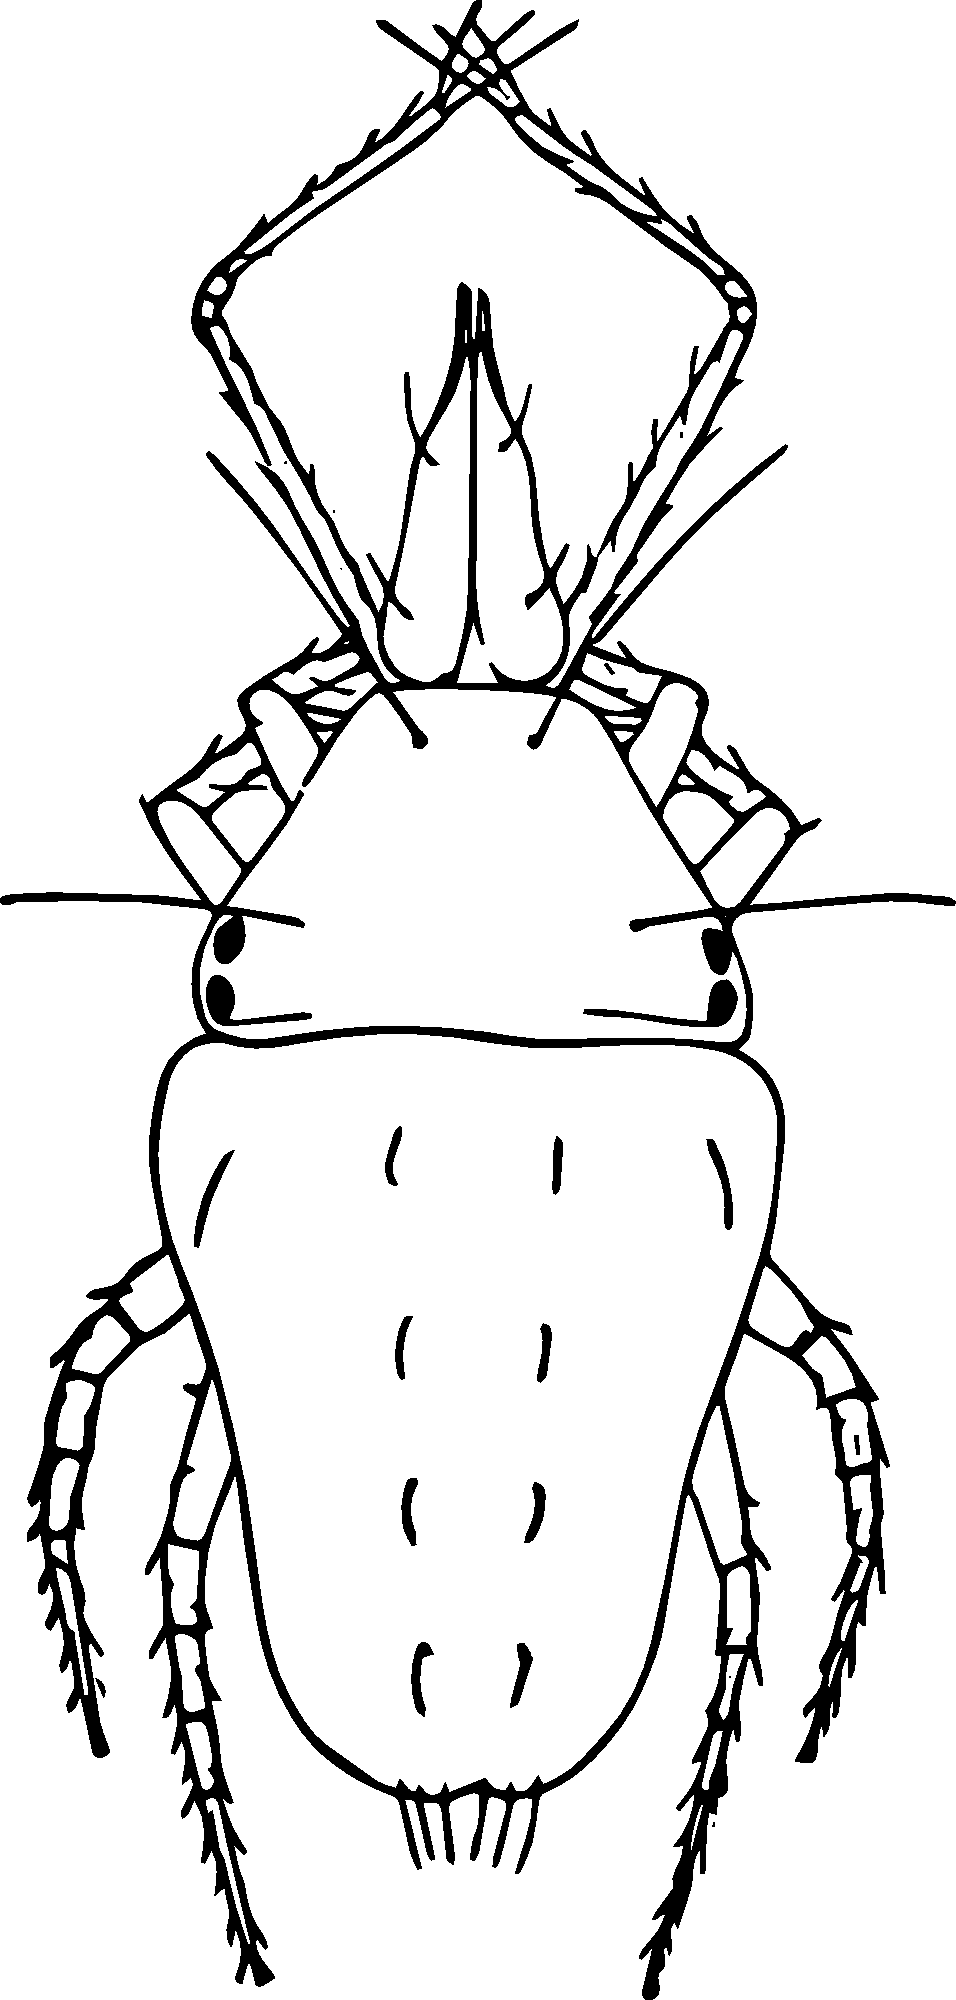
\includegraphics[angle=270,width=\textwidth]{nonhexapod/mite21}
        \caption{}
        \label{fig:mite2}
    \end{subfigure}
    \caption{Mites (Acari). \textbf{(a)} Lateral habitus of oribatid mite \citep[][Fig. 187]{bhlitem132773acari}; \textbf{(b)} dorsal habitus \citep[][Fig. 21]{bhlitem132773acari}} \label{fig:mites}
\end{figure}

\begin{figure}[ht!]
  \centering
    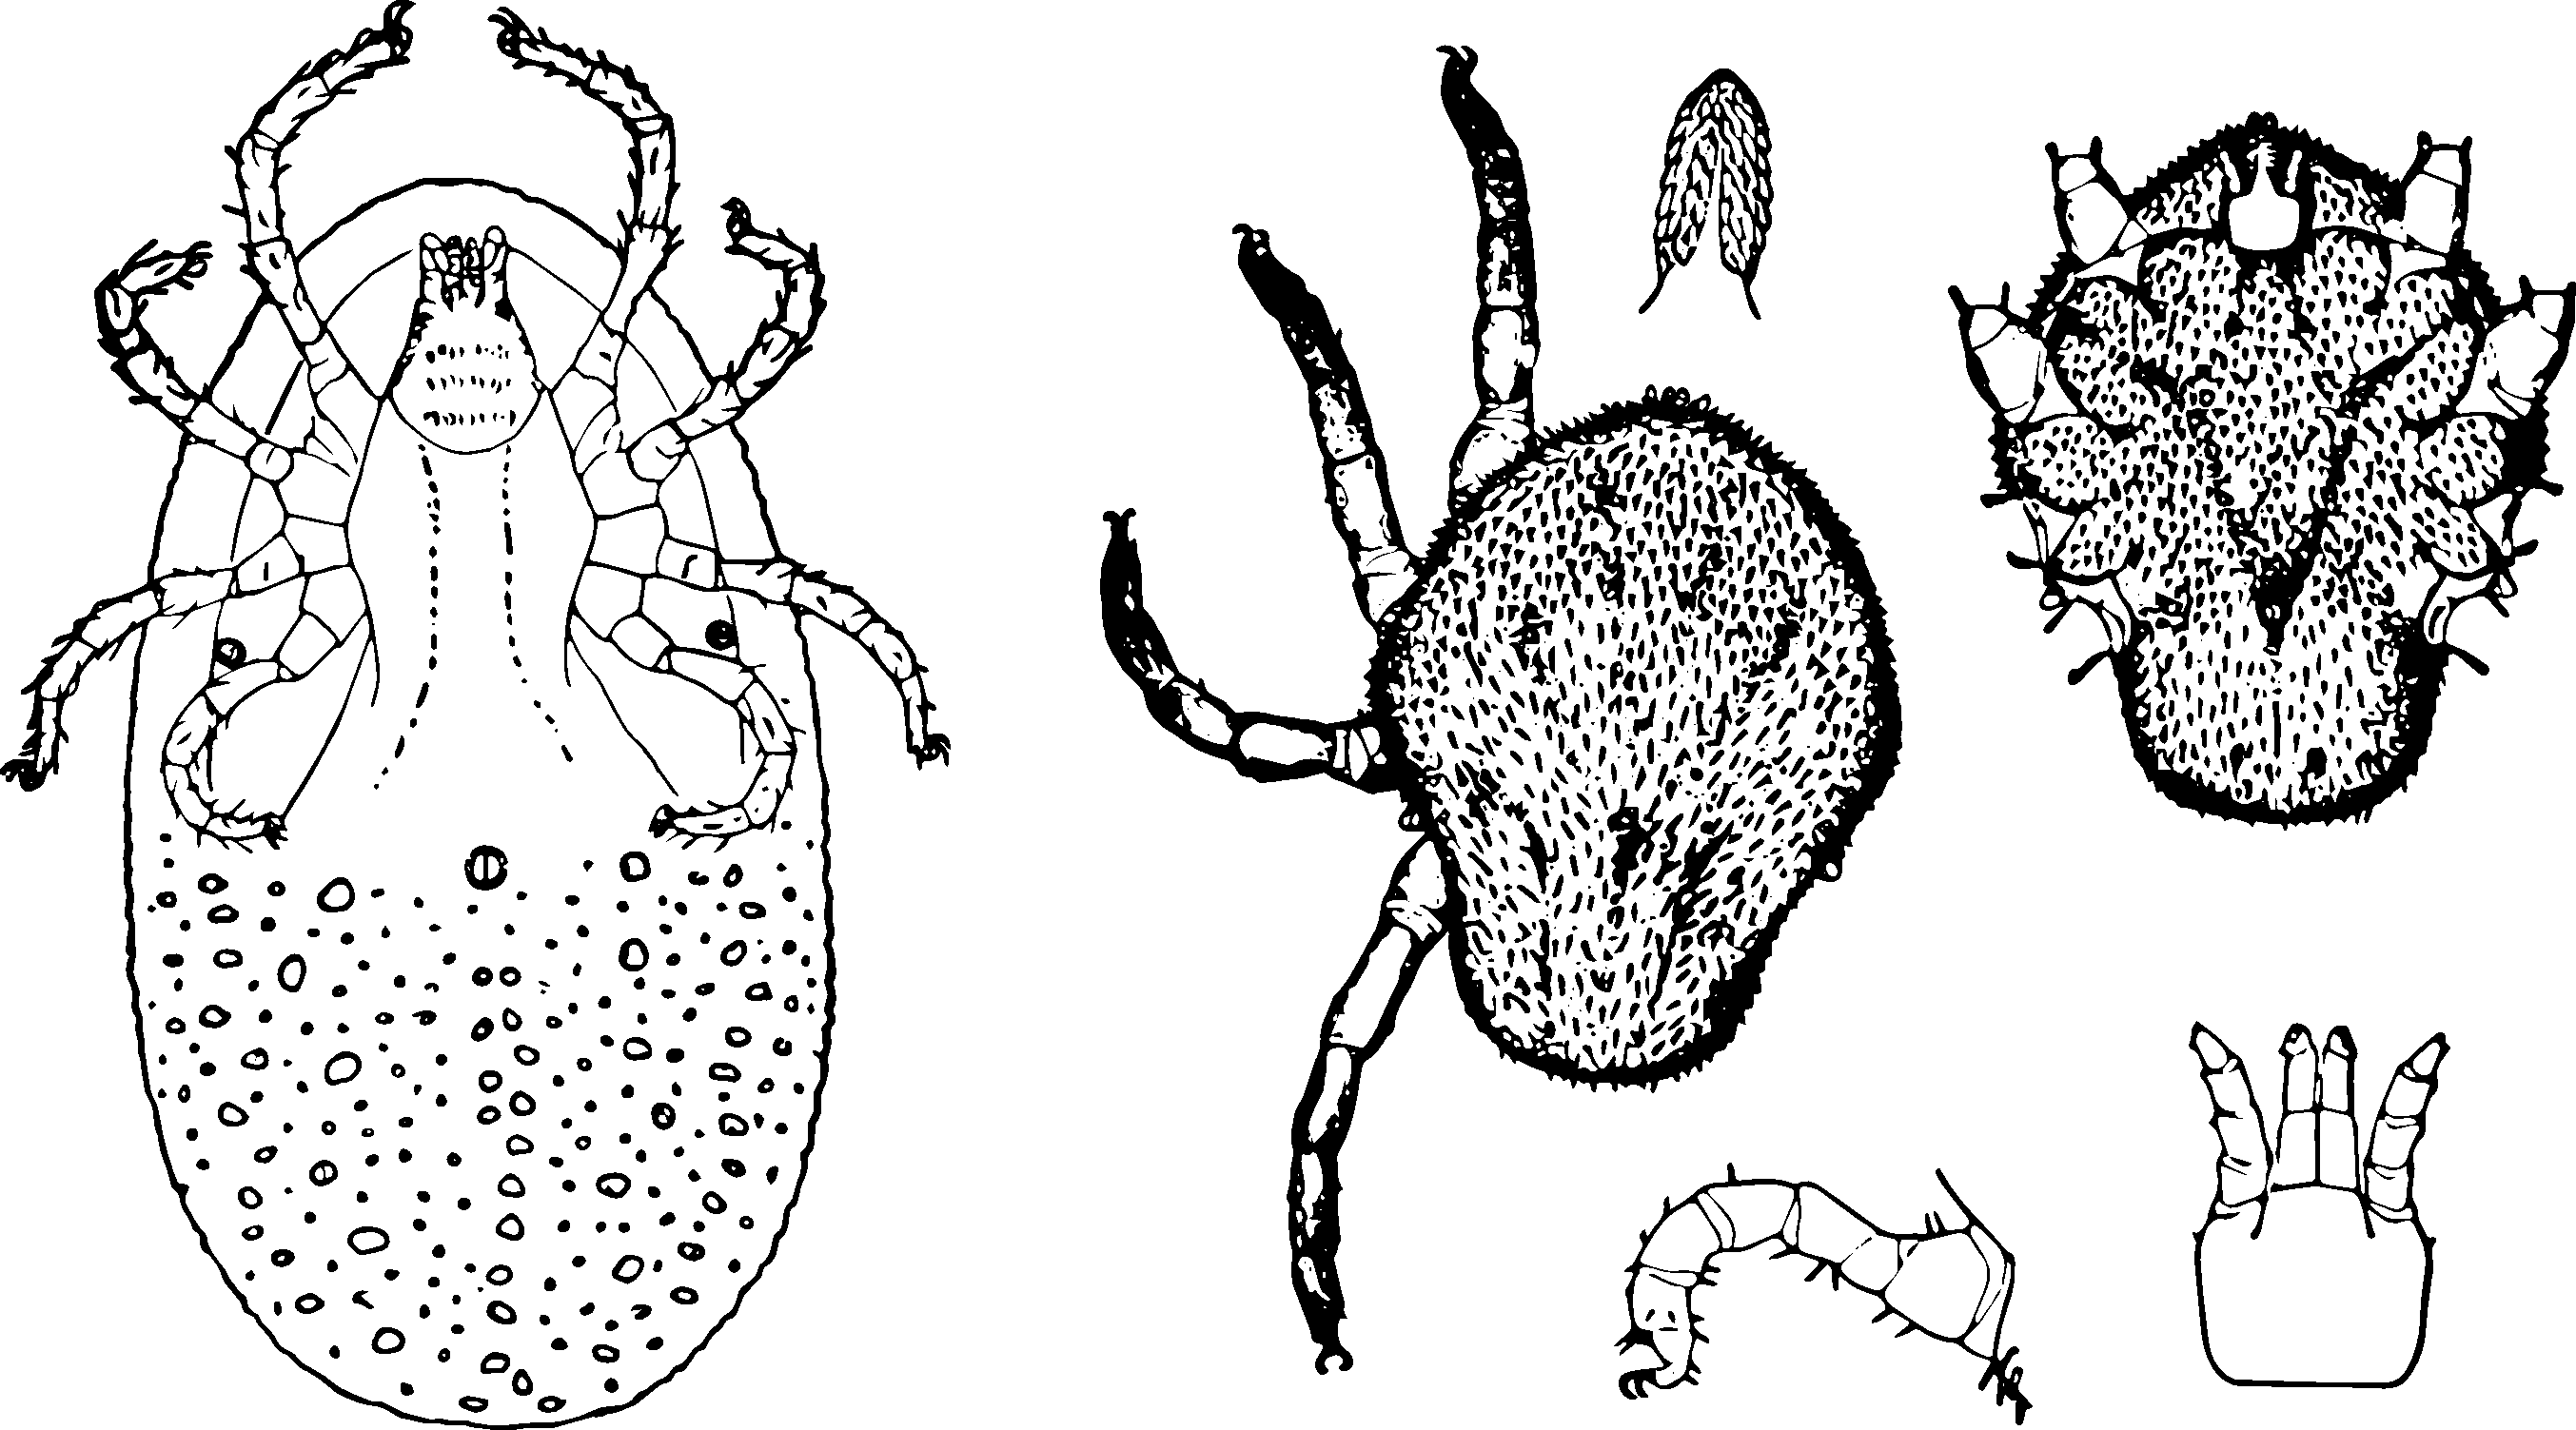
\includegraphics[width=0.65\textwidth]{nonhexapod/ixodid103104}
  \caption{Ticks \citep[][Figs. 103, 104]{bhlitem132773acari}}
  \label{fig:ixodid}
\end{figure}

\subsection{Opiliones (Phalangida, harvestmen, daddy-longlegs)}\index{Opiliones}
\noindent{}\textit{Diagnostic characters:} Chelicerae chelate; opisthosoma segmented, broadly joined to prosoma, without tail-like structure (telson) (figure \ref{fig:opiliones1}); body ovoid; body  \textless7 mm long usually, with leg span up to 160 mm; pedipalp morphology variable: usually thinner than legs, sometimes raptorial.\vspace{3mm}

\noindent{}\textit{Natural history:} Most species are predators and/or scavengers, feeding with a compound structure (stomotheca), formed, in part, by the proximal pedipalp and anteriormost leg segments. These arachnids lack venom and silk glands but do produce noxious defensive odors through scent gland openings (ozopores). There are more than 6,500 species.\vspace{3mm}

\begin{figure}[ht!]
  \centering
    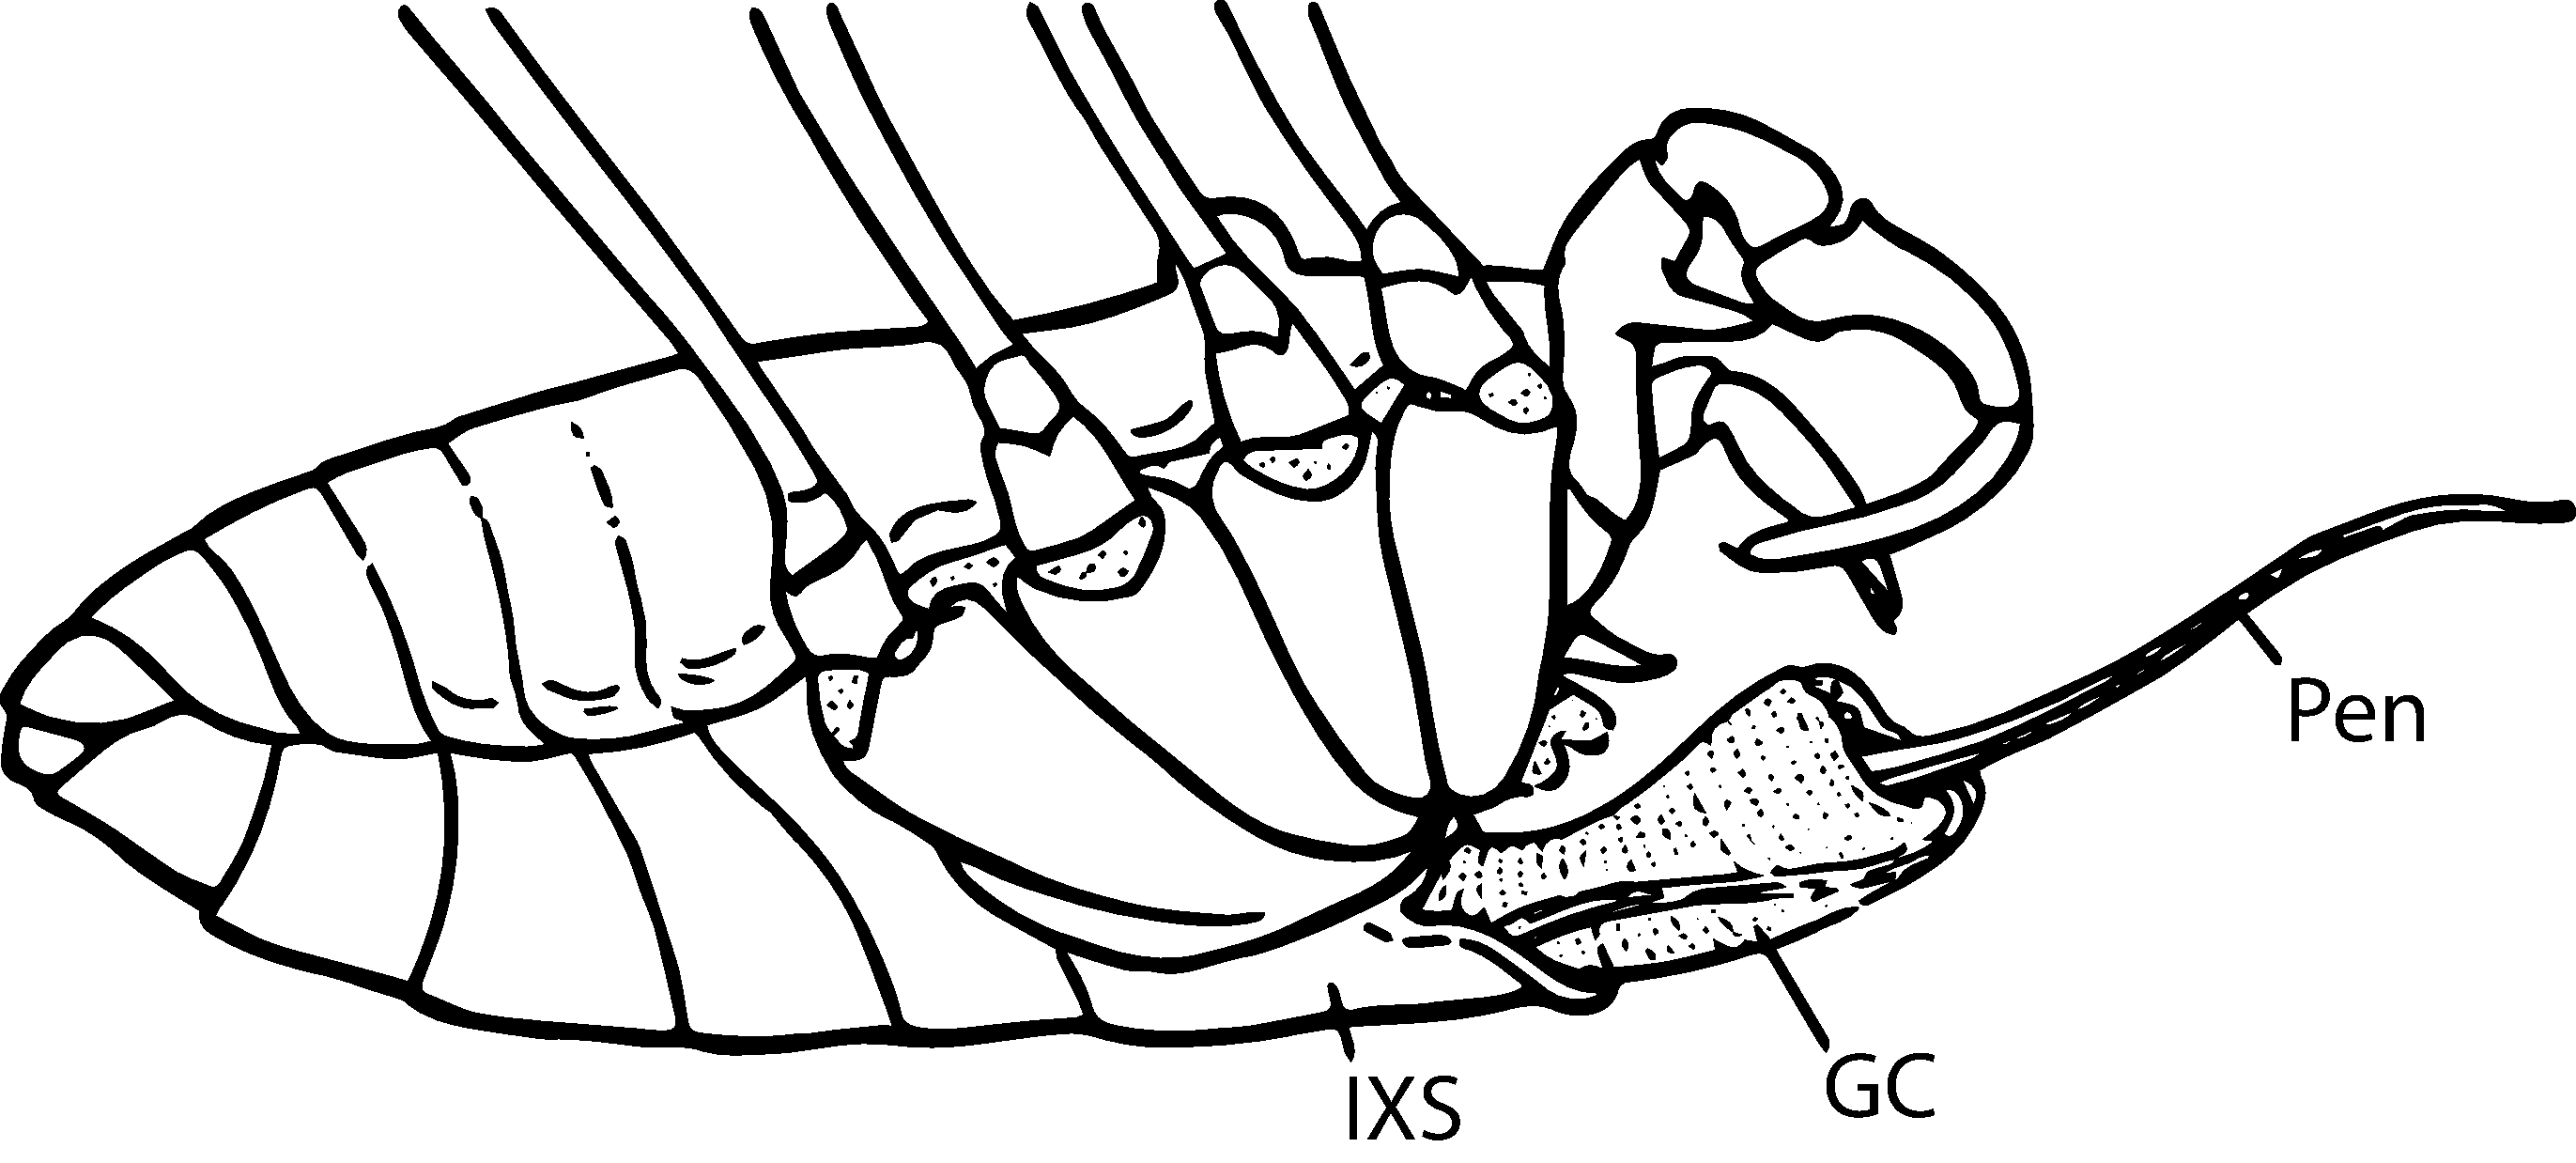
\includegraphics[width=0.6\textwidth]{nonhexapod/opilion12C}
  \caption{Opiliones lateral habitus. Pen = penis; GC = genital chamber; IXS = 9th segment sternum  \citep{snodgrass1937morphology}}
  \label{fig:opiliones1}
\end{figure}

\subsection{Scorpiones (scorpions)}\index{Scorpiones}
\noindent{}\textit{Diagnostic characters:} Chelicerae chelate; pedipalps long, chelate, and usually at least as thick as legs (figure \ref{fig:scorpion}); anteriormost pair of legs used for walking (\textit{i.e.}, not antenniform); opisthosoma segmented, broadly joined to prosoma; tail-like posteriorly (tail = \latinword{telson}); telson with venom gland and \latinword{stinger} present; 2nd segment of opisthosoma with comb-like sensory organs (pectines) ventrally.\vspace{3mm}

\noindent{}\textit{Natural history:} There are more than 1,700 species found worldwide, all of which are predators.\vspace{3mm}

\begin{figure}[ht!]
  \centering
    \includegraphics[width=0.7\textwidth]{nonhexapod/scorpions}
  \caption{Scorpiones \cite[][Plate 18, Figs. 1, 1b, 2]{bhlitem239255}}
  \label{fig:scorpion}
\end{figure}

\begin{theo}
{}Some scorpion species have massive pedipalps and relatively small telsons, while others exhibit the opposite set of phenotypes (\textit{i.e.}, massive telsons but small pedipalps; see figure \ref{fig:scorpion}). From a natural history perspective, what do you think is happening with these structures? Also, how do you think scorpions find prey?
\end{theo} %see https://doi.org/10.3389/fevo.2019.00196 / https://doi.org/10.1371/journal.pone.0078955

\subsection{Pseudoscorpiones (Pseudoscorpionida, Chelonethida, pseudoscorpions)}\index{Pseudoscorpiones}
\noindent{}\textit{Diagnostic characters:} Chelicerae chelate; pedipalps long, chelate, and thicker than legs (figure \ref{fig:pseudo}); anteriormost pair of legs used for walking (\textit{i.e.}, not antenniform); opisthosoma segmented, broadly joined to prosoma, without telson; patellar segment absent on legs.\vspace{3mm}

\noindent{}\textit{Natural history:} There are 3,300 species of pseudoscorpion, most of which are relatively small (\textless5 mm long). Sometimes they can be found clinging to insects, hitching a ride (phoresy) or possibly eating parasitic mites (phagophilia). Some species subdue prey with venom, from a gland in the pedipalp.\vspace{3mm}

\begin{figure}[ht!]
  \centering
    \includegraphics[width=0.4\textwidth]{nonhexapod/pseudoscorppl4fig6}
  \caption{Pseudoscorpiones \citep[][Plate IV, Fig. 6]{bhlitem260979pseudo}}
  \label{fig:pseudo}
\end{figure}

\section{Myriapoda}\index{Myriapoda}
\begin{itemize}
\item antennae present as single pair
\item appendages uniramous (\textit{i.e.}, no branches)
\item mouthparts mandibulate (\textit{i.e.}, not chelicerate)
\end{itemize}

\subsection{Diplopoda (millipedes)}\index{Diplopoda}
\noindent{}\textit{Diagnostic characters:} Most (apparent) segments with 2 pairs of legs (figure \ref{fig:diplop2}); antennae usually 7-segmented, short; 30+ pairs of legs present usually; body usually round, tube-like; some species small, bristly (figure \ref{fig:diplop1}).\vspace{3mm}

\noindent{}\textit{Natural history:} Millipedes typically forage on rotting materials (saprophagy) and are important recyclers of nutritive material. Most species are harmless, although some are renown for excreting toxic compounds when handled. There are \textgreater12,000 species described worldwide.\vspace{3mm}

\begin{figure}[ht!]
    \centering
    \begin{subfigure}[ht!]{0.27\textwidth}
        \includegraphics[width=\textwidth]{nonhexapod/diplopod82}
        \caption{}
        \label{fig:diplop1}
    \end{subfigure}
    \hfill
    \begin{subfigure}[ht!]{0.65\textwidth}
        \includegraphics[width=\textwidth]{nonhexapod/millip}
        \caption{}
        \label{fig:diplop2}
    \end{subfigure}
    \caption{Millipedes (Diplopoda). \textbf{(a)} Bristle millipede (Polyxenida) \citep[][Fig. 82]{bhlitem40112britmus}; \textbf{(b)} Diplopoda \citep{bhlitem94979diplopo}} \label{fig:diplopoda}
\end{figure}

\subsection{Chilopoda (centipedes)}\index{Chilopoda}
\noindent{}\textit{Diagnostic characters:} Antennae usually with 14+ segments; apices of anteriormost pair of legs (\latinword{forcipules}) modified into fang-like structures (figure \ref{fig:chilo2}); most segments with 1 pair of legs; 15+ pairs of legs present usually (figure \ref{fig:chilo2}); body usually dorsoventrally flattened.\vspace{3mm}

\noindent{}\textit{Natural history:} These arthropods are predators of other organisms, including, in some cases, vertebrates. Prey are subdued with venom from the forcipules.\vspace{3mm}


\begin{figure}[ht!]
	\centering
        \includegraphics[width=0.8\textwidth]{nonhexapod/chilopod}
        \caption{Chilopoda. Modified from Fig. 138 in \cite{bhlitem91180chilopod} and, top left, Fig. 192 in \cite{bhlitem117775chilo2}}
        \label{fig:chilo2}
\end{figure}

\begin{theo}
{}Why do myriapods have so many legs? What advantage(s) does this condition provide these arthropods?
\end{theo}

\section{Non-hexapod Pancrustacea (formerly ``Crustacea'')}\index{Crustacea}\index{Pancrustacea}
\begin{itemize}
\item often with 2 tagmata: cephalothorax and abdomen
\item many biramous (2-branched) appendages, usually with 2nd pair of antennae (antennules)
\item mouthparts mandibulate
\end{itemize}

\subsection{Isopoda (pillbugs, sowbugs)}\index{Isopoda}
\noindent{}\textit{Diagnostic characters:} Body with no carapace, usually dorso-ventrally flattened (figure \ref{fig:isopod2}); 7 pairs of thoracic legs; 2nd pair of antennae reduced.\vspace{3mm}

\noindent{}\textit{Natural history:} One of the few non-hexapod pancrustaceans to radiate in the terrestrial environment. Of the approximately 10,000 known species, about half are terrestrial. The rest are marine (about 4,500 spp.) or inhabit freshwater. Most species survive as scavengers but many are parasitic on fish or other aquatic organisms.\vspace{3mm}

\subsection{Amphipoda (scuds)}\index{Amphipoda}
\noindent{}\textit{Diagnostic characters:} No carapace, usually laterally flattened (figure \ref{fig:amphip}); fore legs often raptorial; usually 6 or 7 pairs of thoracic legs.\vspace{3mm}

\noindent{}\textit{Natural history:} Of the 9,500 known species, approximately 20\% are found in freshwater. The vast majority are marine, but a handful are terrestrial (usually closely associated with aquatic habitats). They are mostly scavengers.\vspace{3mm}

\begin{figure}[ht!]
    \centering
    \begin{subfigure}[ht!]{0.4\textwidth}\reflectbox{
        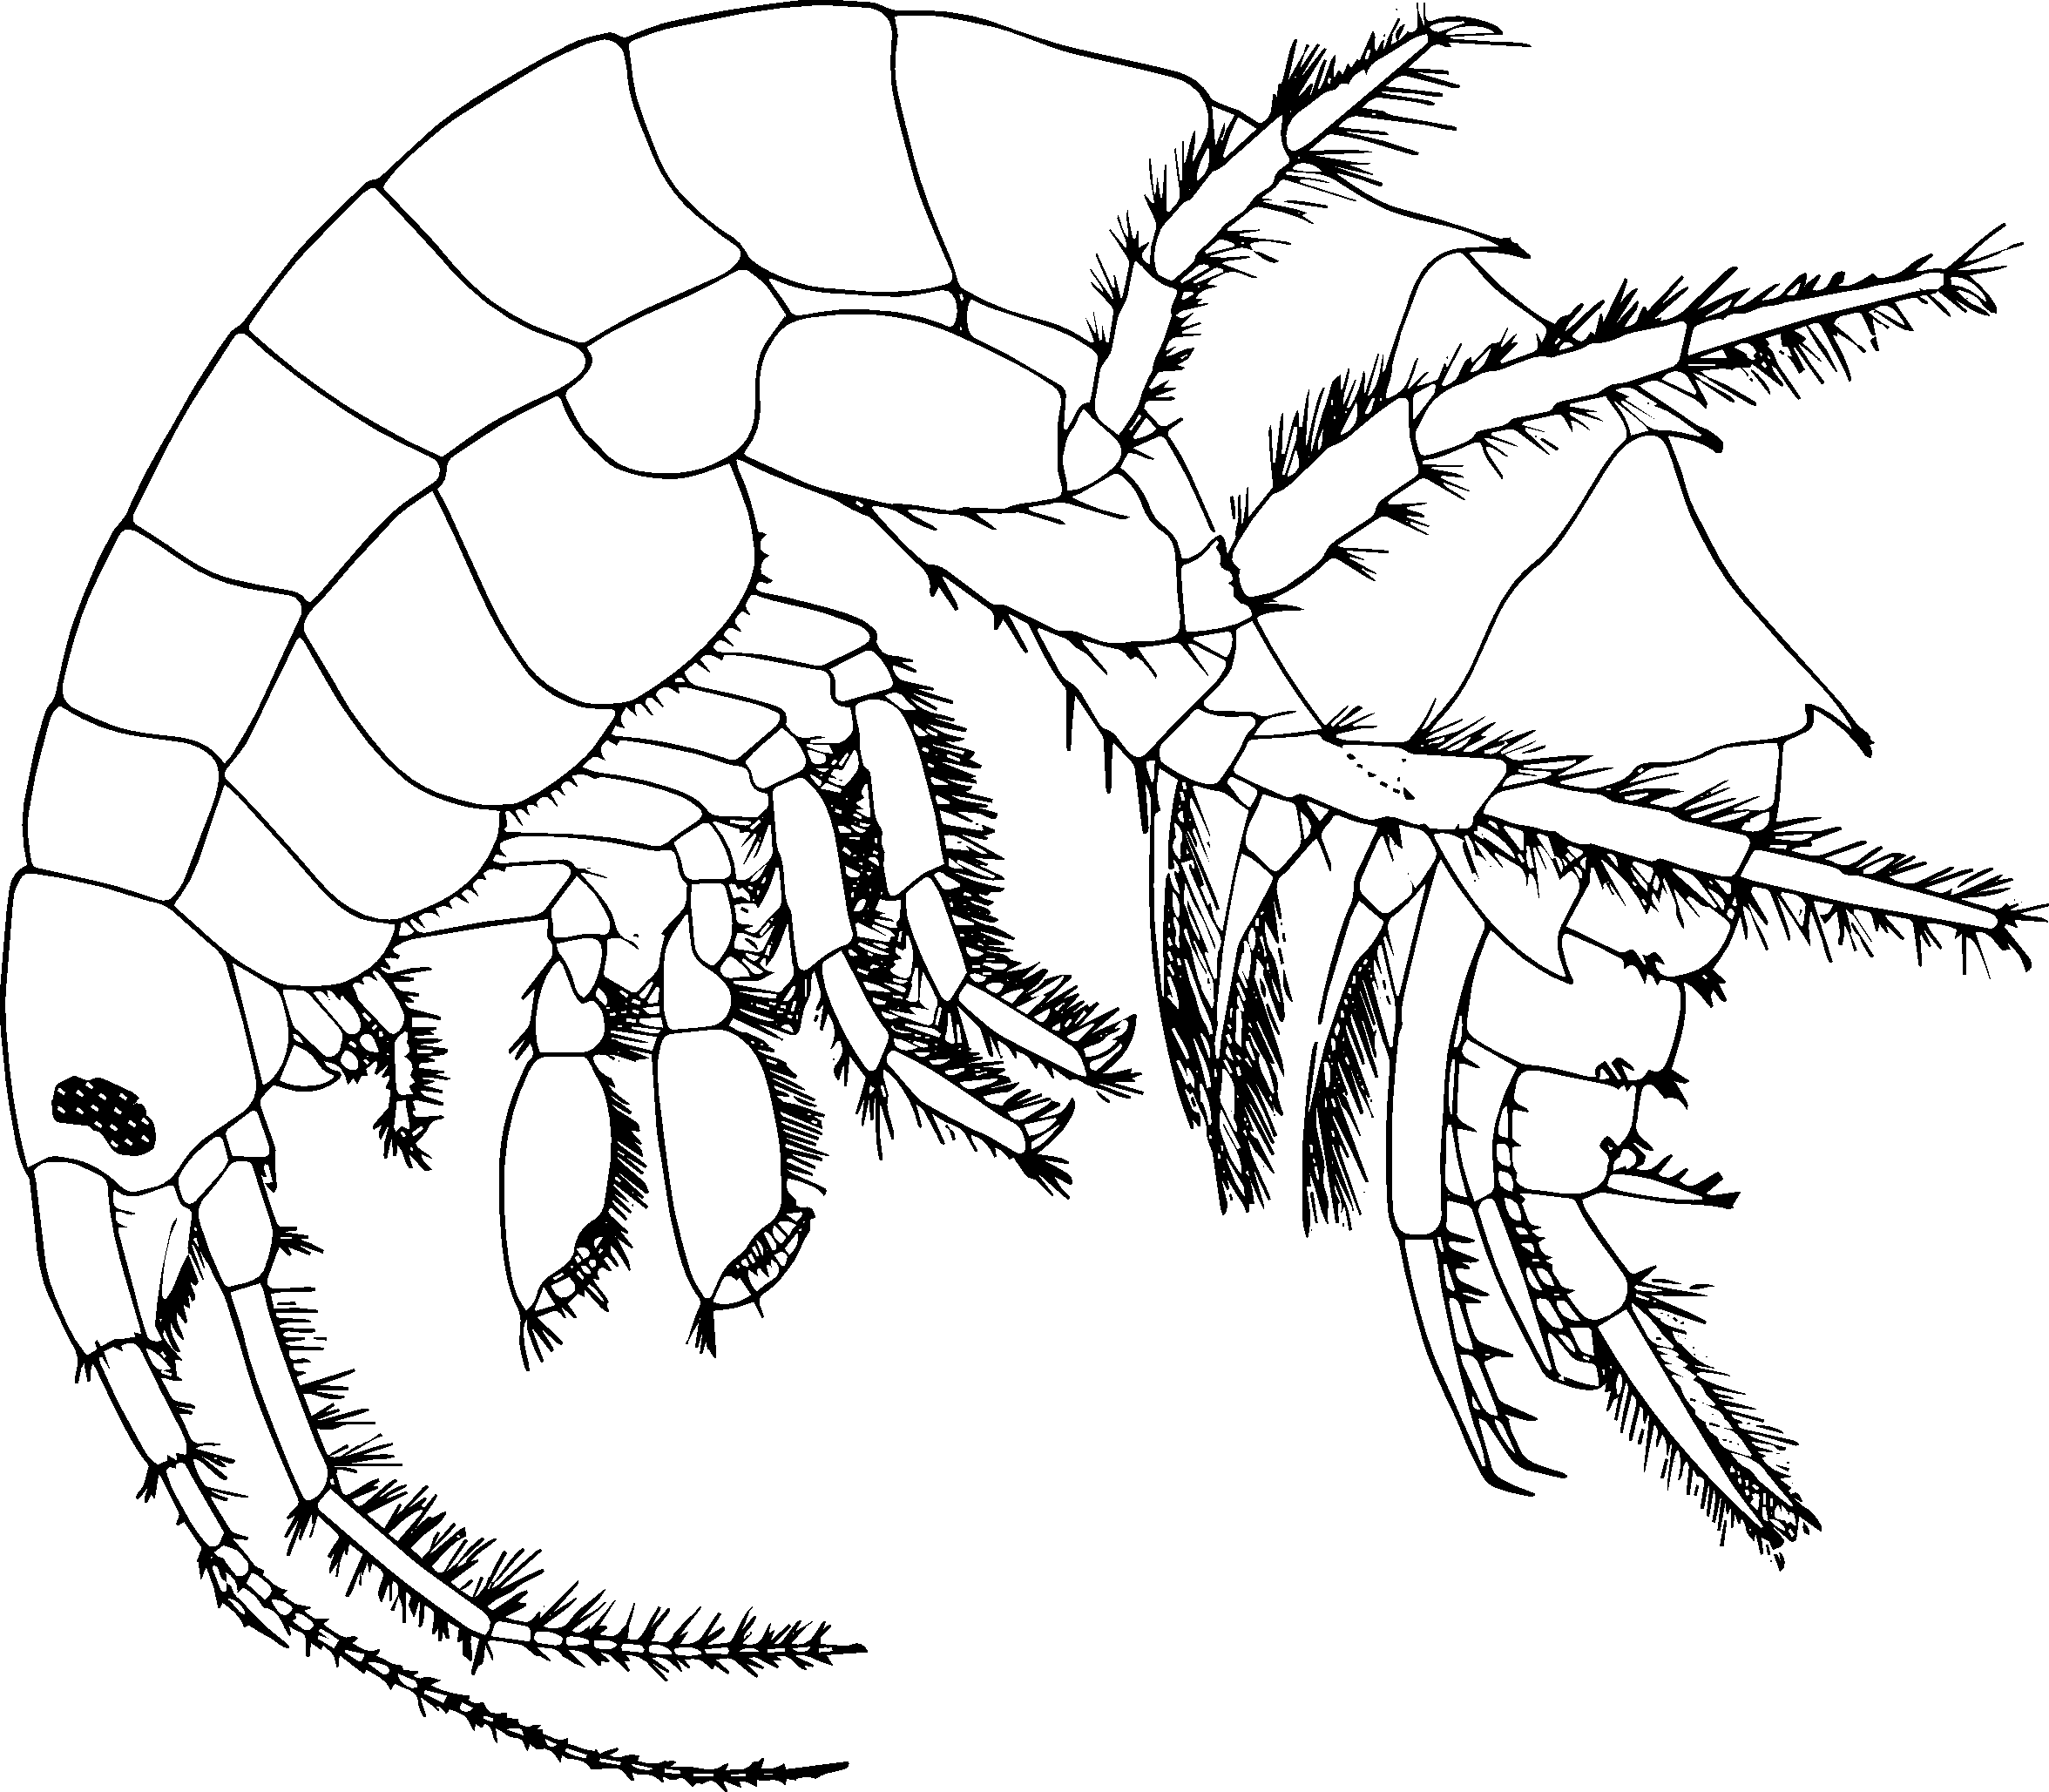
\includegraphics[width=\textwidth]{nonhexapod/amphipod30}}
        \caption{Amphipoda \citep[][Fig. 30]{bhlitem148531crust}}
        \label{fig:amphip}
    \end{subfigure}
    \hfill 
    \begin{subfigure}[ht!]{0.45\textwidth}
        \includegraphics[angle=270,width=\textwidth]{nonhexapod/isopod55}
        \caption{Isopoda \citep[][Fig. 55]{bhlitem148531crust}}
        \label{fig:isopod2}
    \end{subfigure}
    \caption{``Crustacea''} 
\end{figure}

\subsection{Branchiopoda (fairy shrimp, clam shrimp)}\index{Branchiopoda}
\noindent{}\textit{Diagnostic characters:} Very diverse in habitus but usually with many appendages, each of which typically has a gill associated with it. Carapace usually prominent (figure \ref{fig:branchiopoda}), either as a shield-like sclerite or even as a hinged, bivalve-like sclerite.\vspace{3mm}

\noindent{}\textit{Natural history:} Aquatic but extraordinarily diverse in natural history. Typically feed on plankton and suspended organic matter, but some are predators and/or scavengers. Many species found in freshwater, and those that inhabit saline or brackish water are usually in continental water bodies (rather than in the ocean). Eggs of many species are capable of weathering hostile environments.\vspace{3mm}

\begin{figure}[ht!]
  \centering
    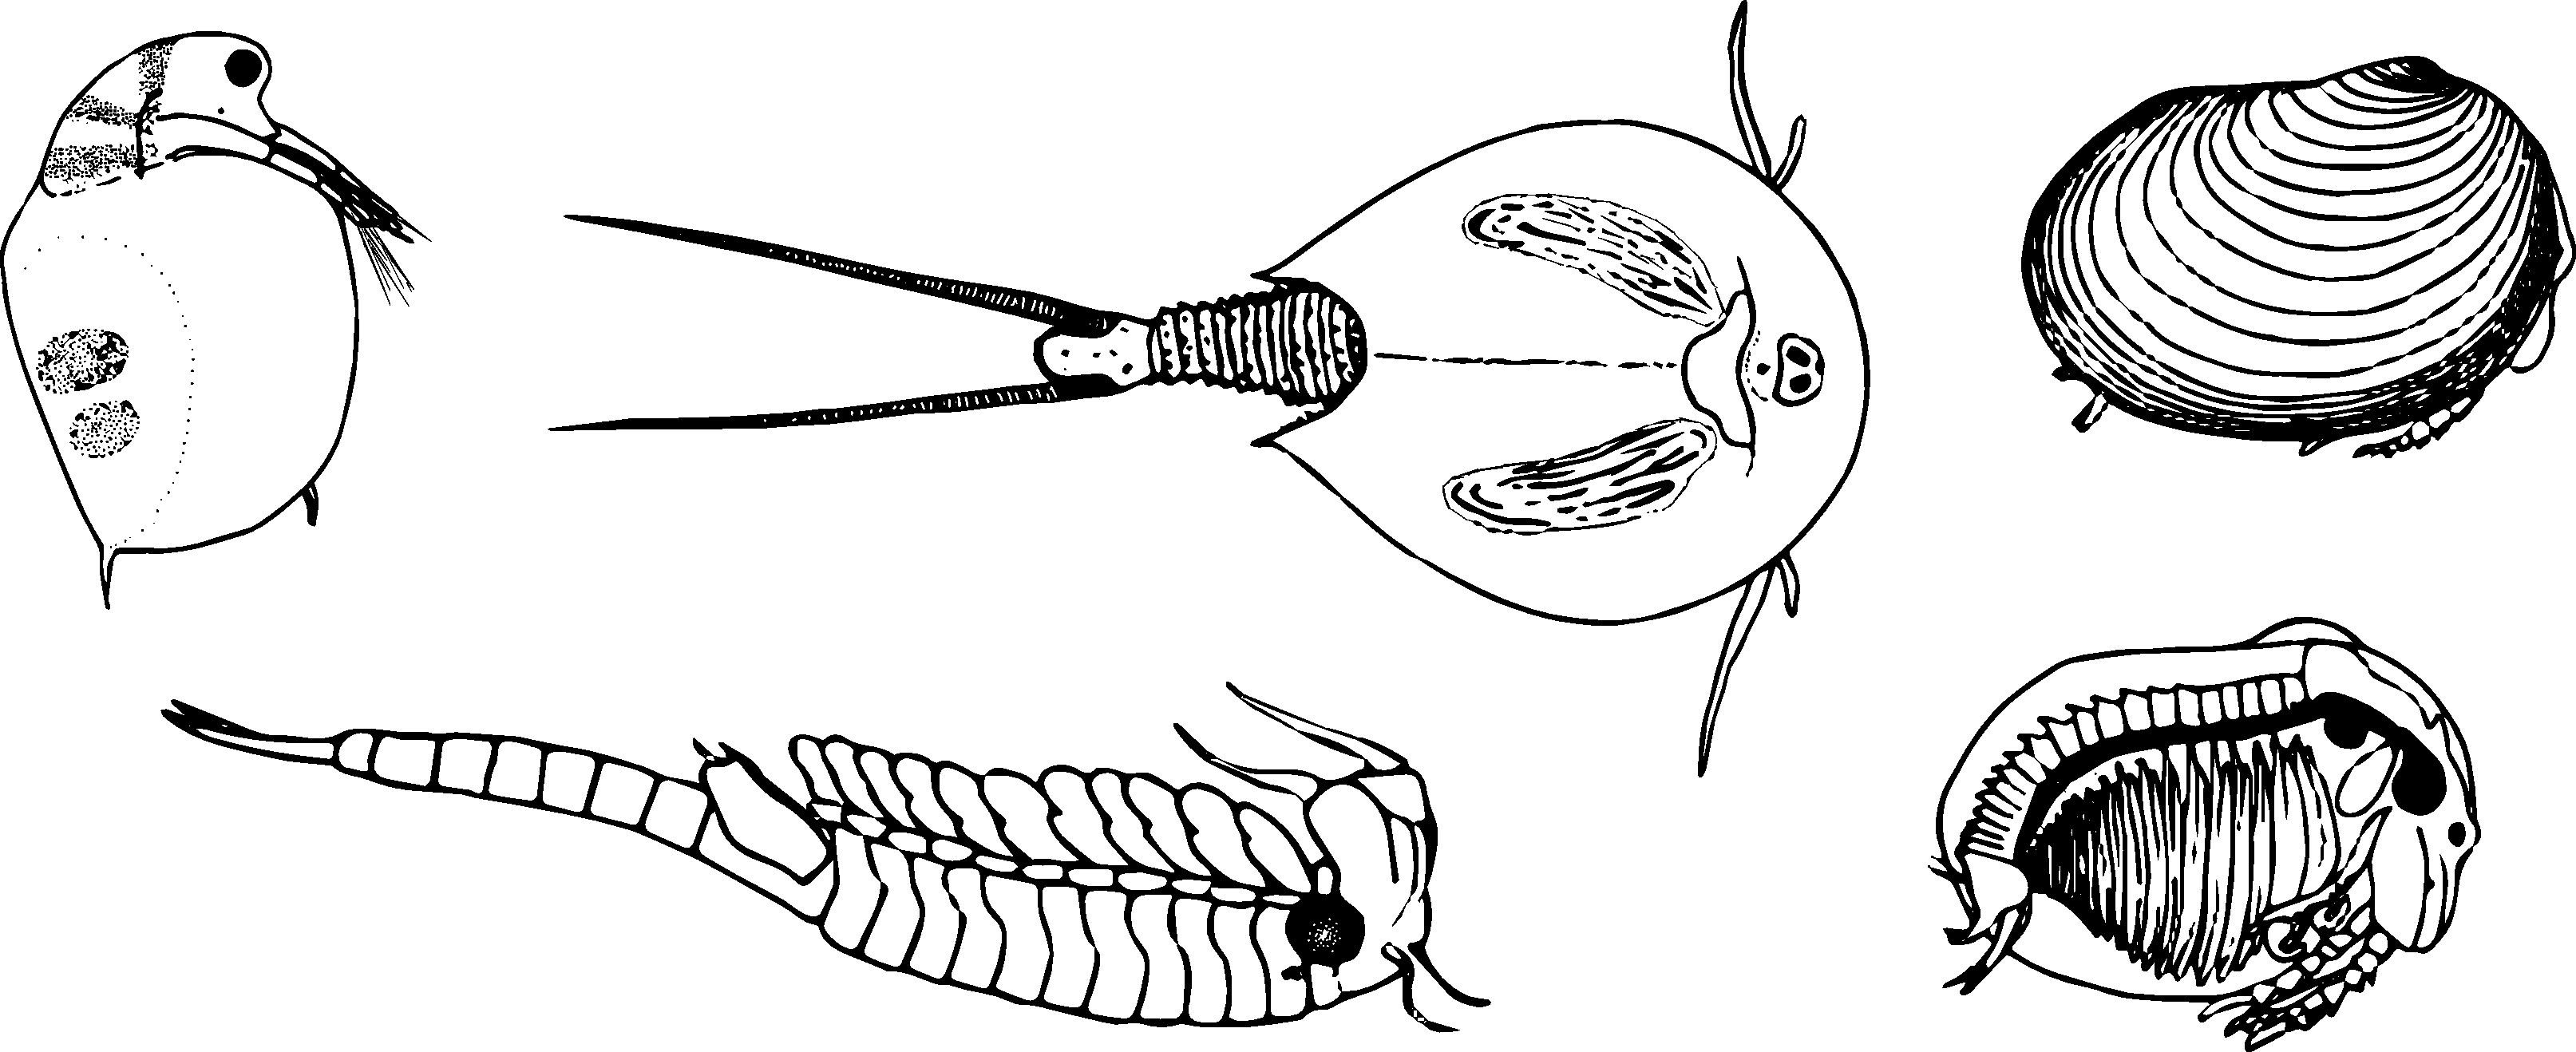
\includegraphics[width=0.8\textwidth]{sections/img/nonhexapod/branchiopoda.pdf}
  \caption{Branchiopoda. redrawn from image at \url{https://web.archive.org/web/20230201062324/https://www.abdn.ac.uk/geosciences/departments/geology/crustaceans-1952.php}}
  \label{fig:branchiopoda}
\end{figure}

\section*{Become a taxonomist}% prob do not need to test on these taxa; could be there simply as demonstrations of the diversity

You've now seen a handful of arthropod taxa, from three groups that are not insects. These organisms are incredibly diverse and remain relevant to understanding the evolution of Arthropoda. Take some time to observe specimens of taxa not covered above, bask in the diversity of their phenotypes, and see if you can classify them correctly. Are they chelicerates, myriapods, or pancrustaceans? Why or why not? Draw and/or describe features you think are diagnostic. Based on their morphology, can you predict their natural history?

\subsubsection*{Solifugae (Solpugida; camelspiders, sunspiders, windscorpions)}\index{Solifugae}
Which major group---Chelicerata, Myriapoda, Pancrustacea---does it belong in and why? What diagnostic characters separate it from the taxa above? What do these arthropods eat, and how do they live?\vspace{3mm}

\begin{figure}[ht!]
  \centering
    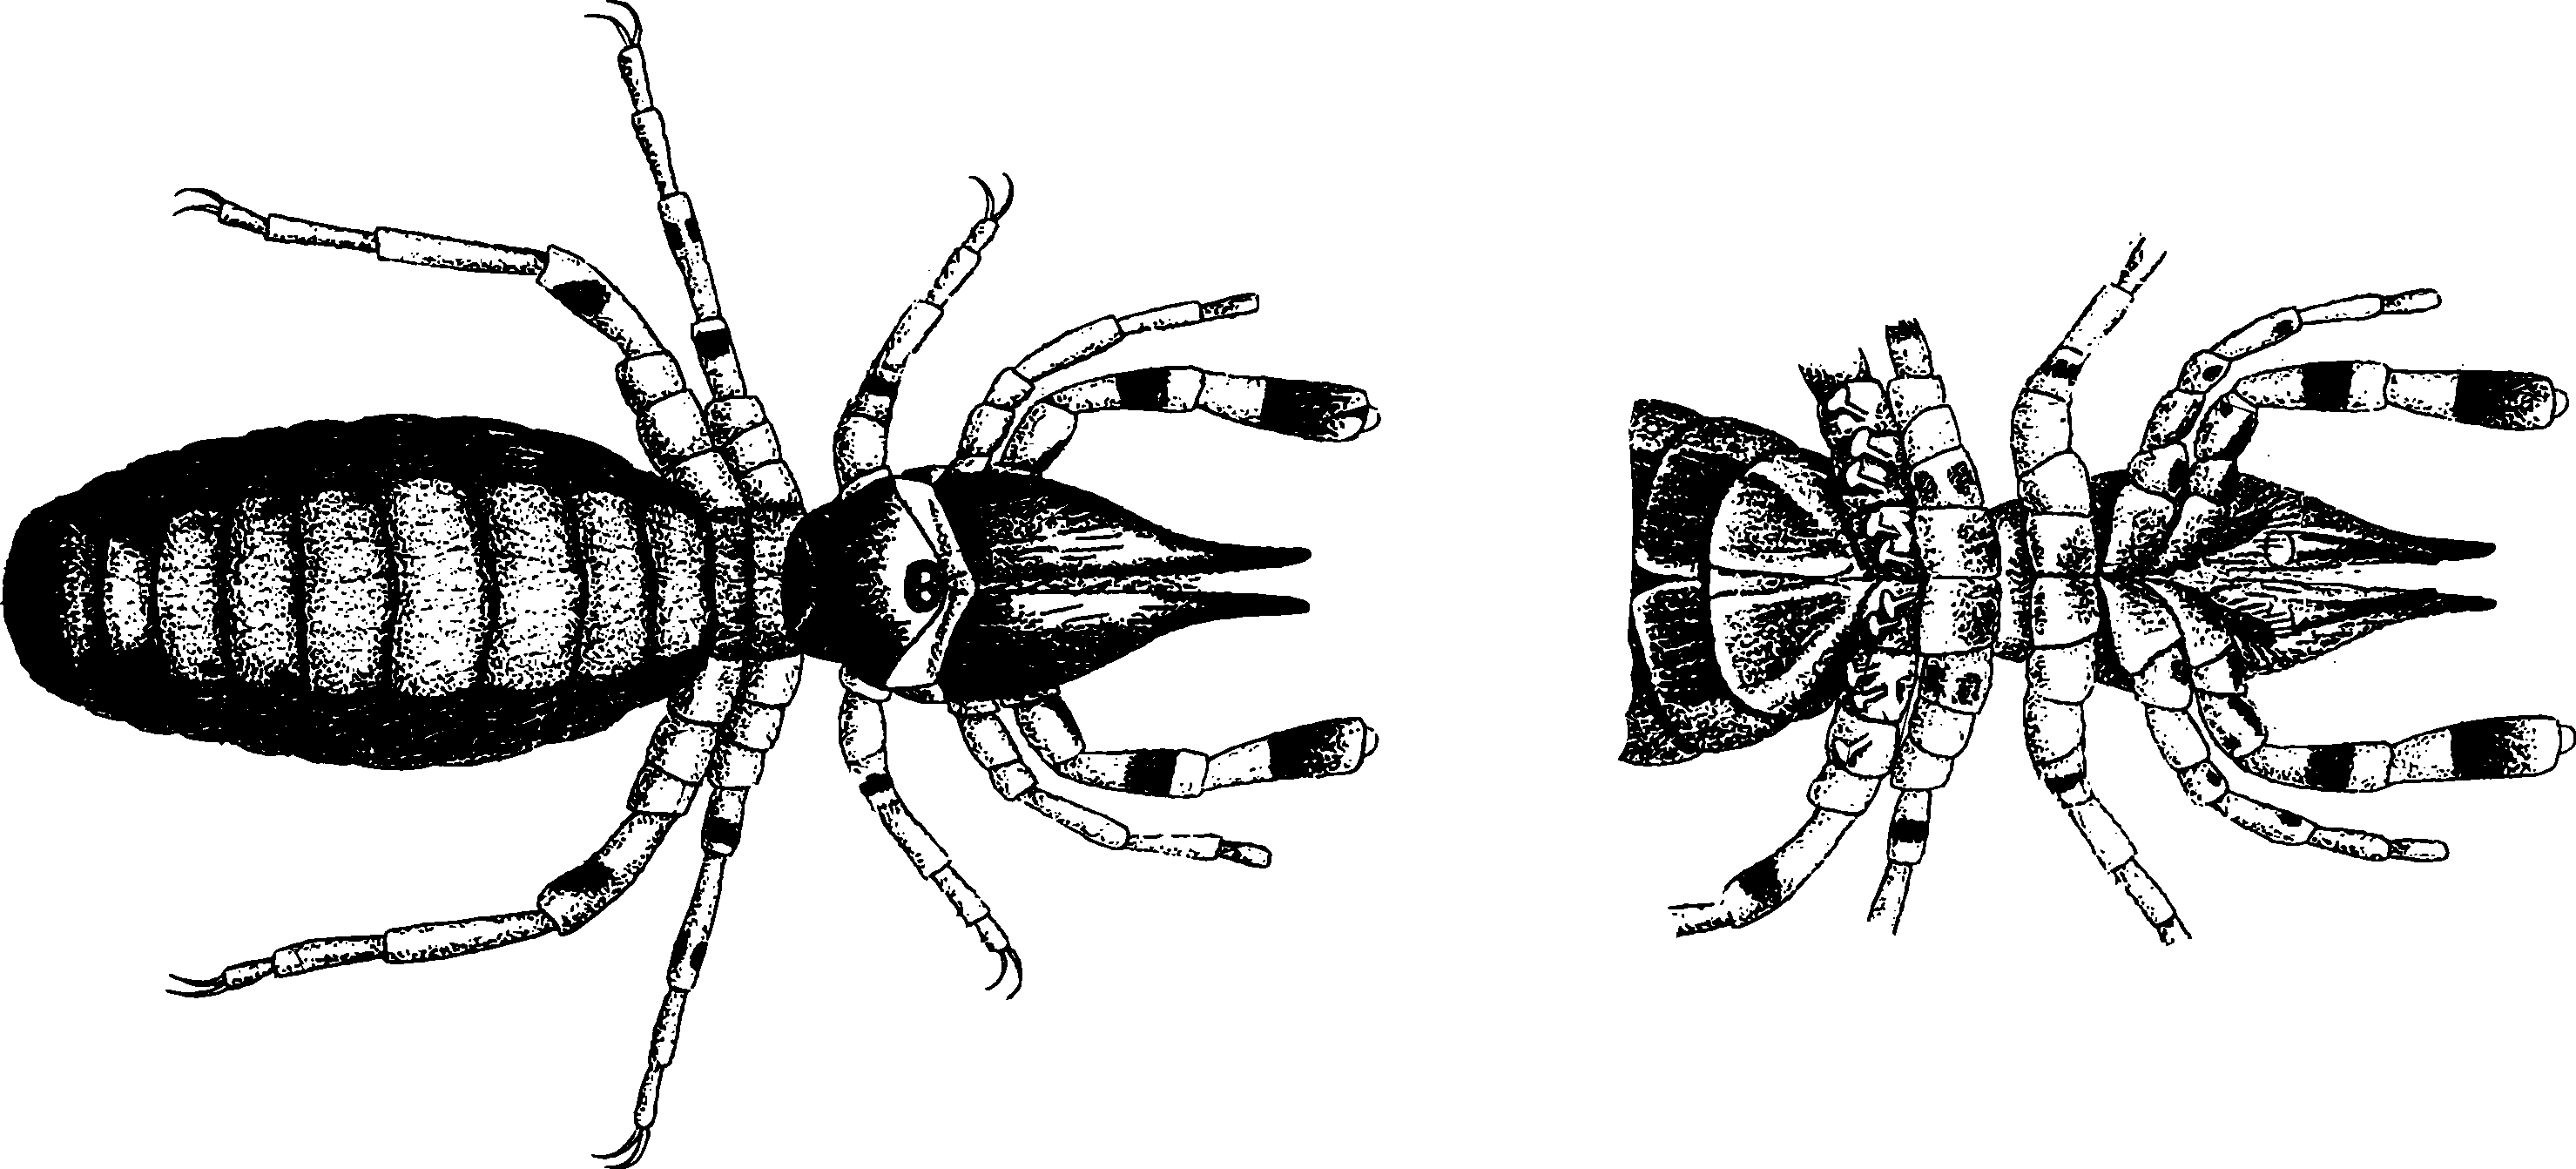
\includegraphics[width=0.8\textwidth]{nonhexapod/solifugae}
  \caption{Solifugae \citep[modified from][Plate 26, Fig. 2]{Bernard1894solifugae}}
  \label{fig:solfugida}
\end{figure}

\subsubsection*{Decapoda (crabs, lobsters, shrimp)}\index{Decapoda}
Which major group does it belong in and why? What diagnostic characters separate it from other taxa in the same group? What do these arthropods eat, and how do they live?\vspace{3mm}

\begin{figure}[ht!]
  \centering
    \includegraphics[width=0.6\textwidth]{nonhexapod/decapod}
  \caption{Decapoda \citep[][Plate VII]{bhlitem114131}}
  \label{fig:decapoda}
\end{figure}

\subsubsection*{Thelyphonida (Uropygi, Uropygida, vinegaroons, whipscorpions)}\index{Thelyphonida}
Which major group does it belong in and why? What diagnostic characters separate it from the other taxa in that group? See figure \ref{fig:thelyphonida}. What do these arthropods eat, and how do they live?\vspace{3mm}

\begin{figure}[ht!]
  \centering
    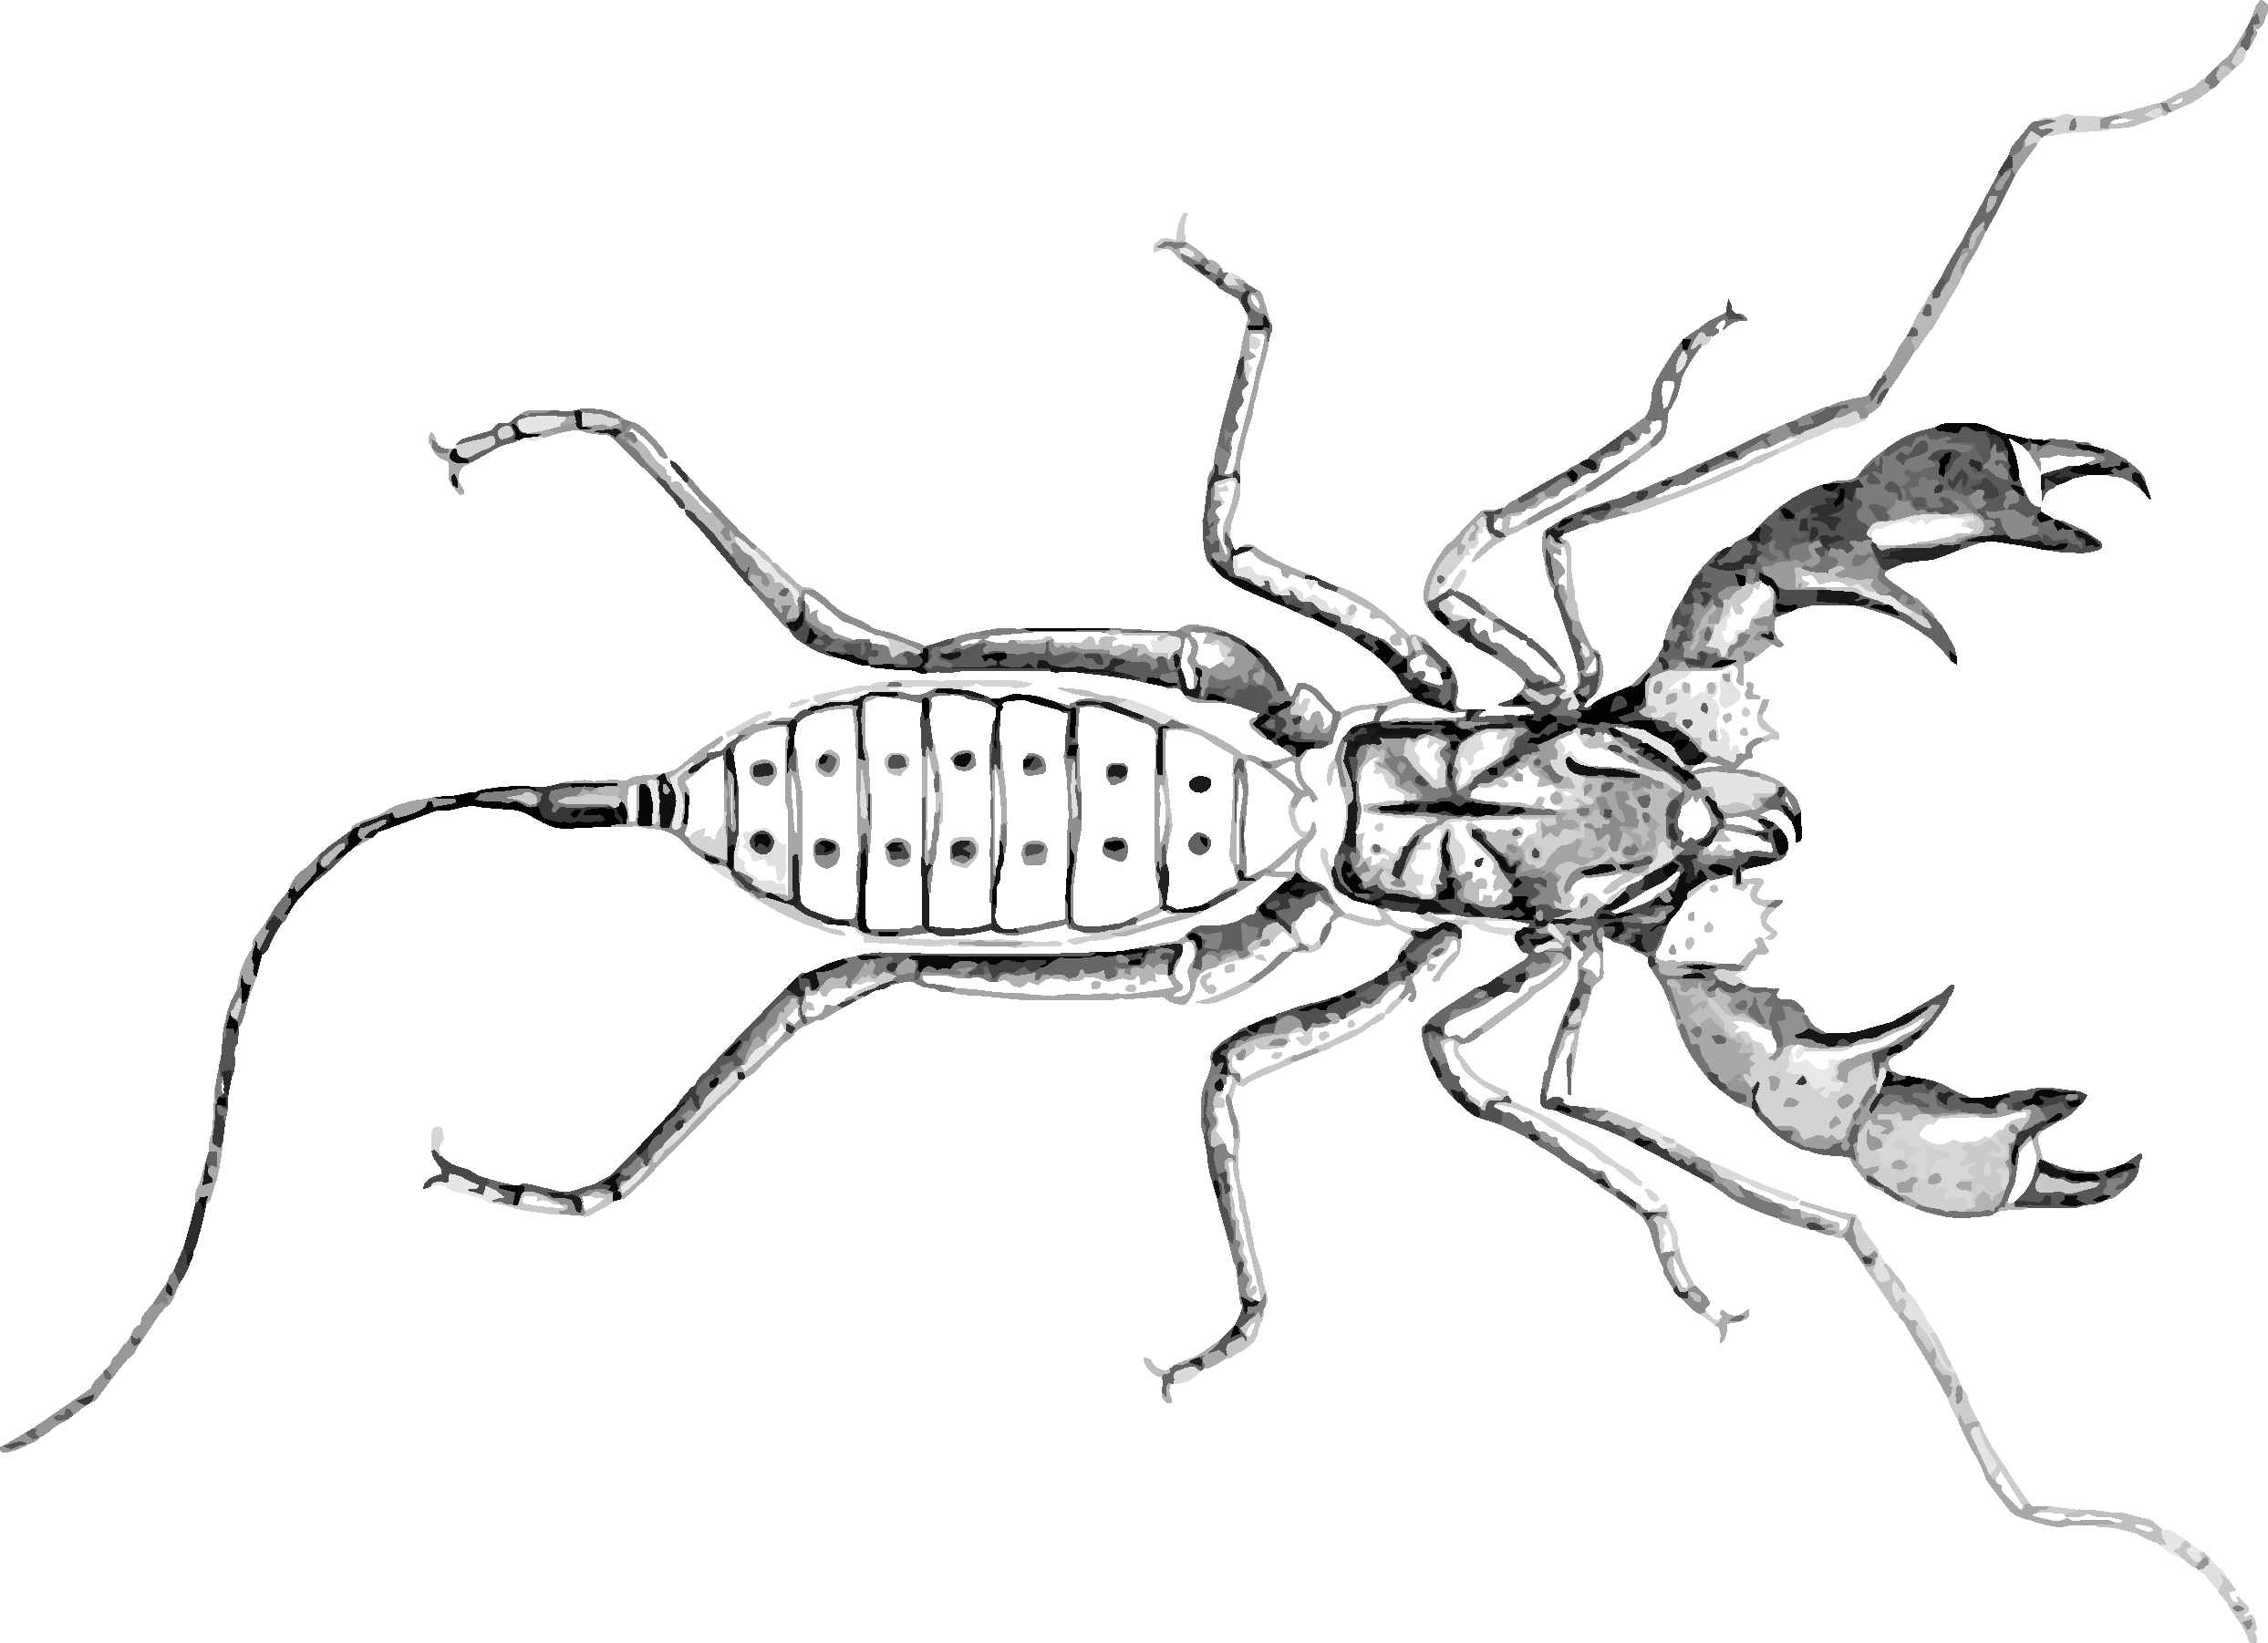
\includegraphics[width=0.5\textwidth]{nonhexapod/thelyphonida}
  \caption{Thelyphonida \citep[][Fig. 57]{bhlitem40112britmus}}
  \label{fig:thelyphonida}
\end{figure}

\subsubsection*{Amblypygi (tail-less whipscorpions)}\index{Amblypygi}
Which major group does it belong in and why? What diagnostic characters separate it from other taxa in that group? See figure \ref{fig:ambly1}. What do these arthropods eat, and how do they live?\vspace{3mm}

\begin{figure}[ht!]
  \centering
    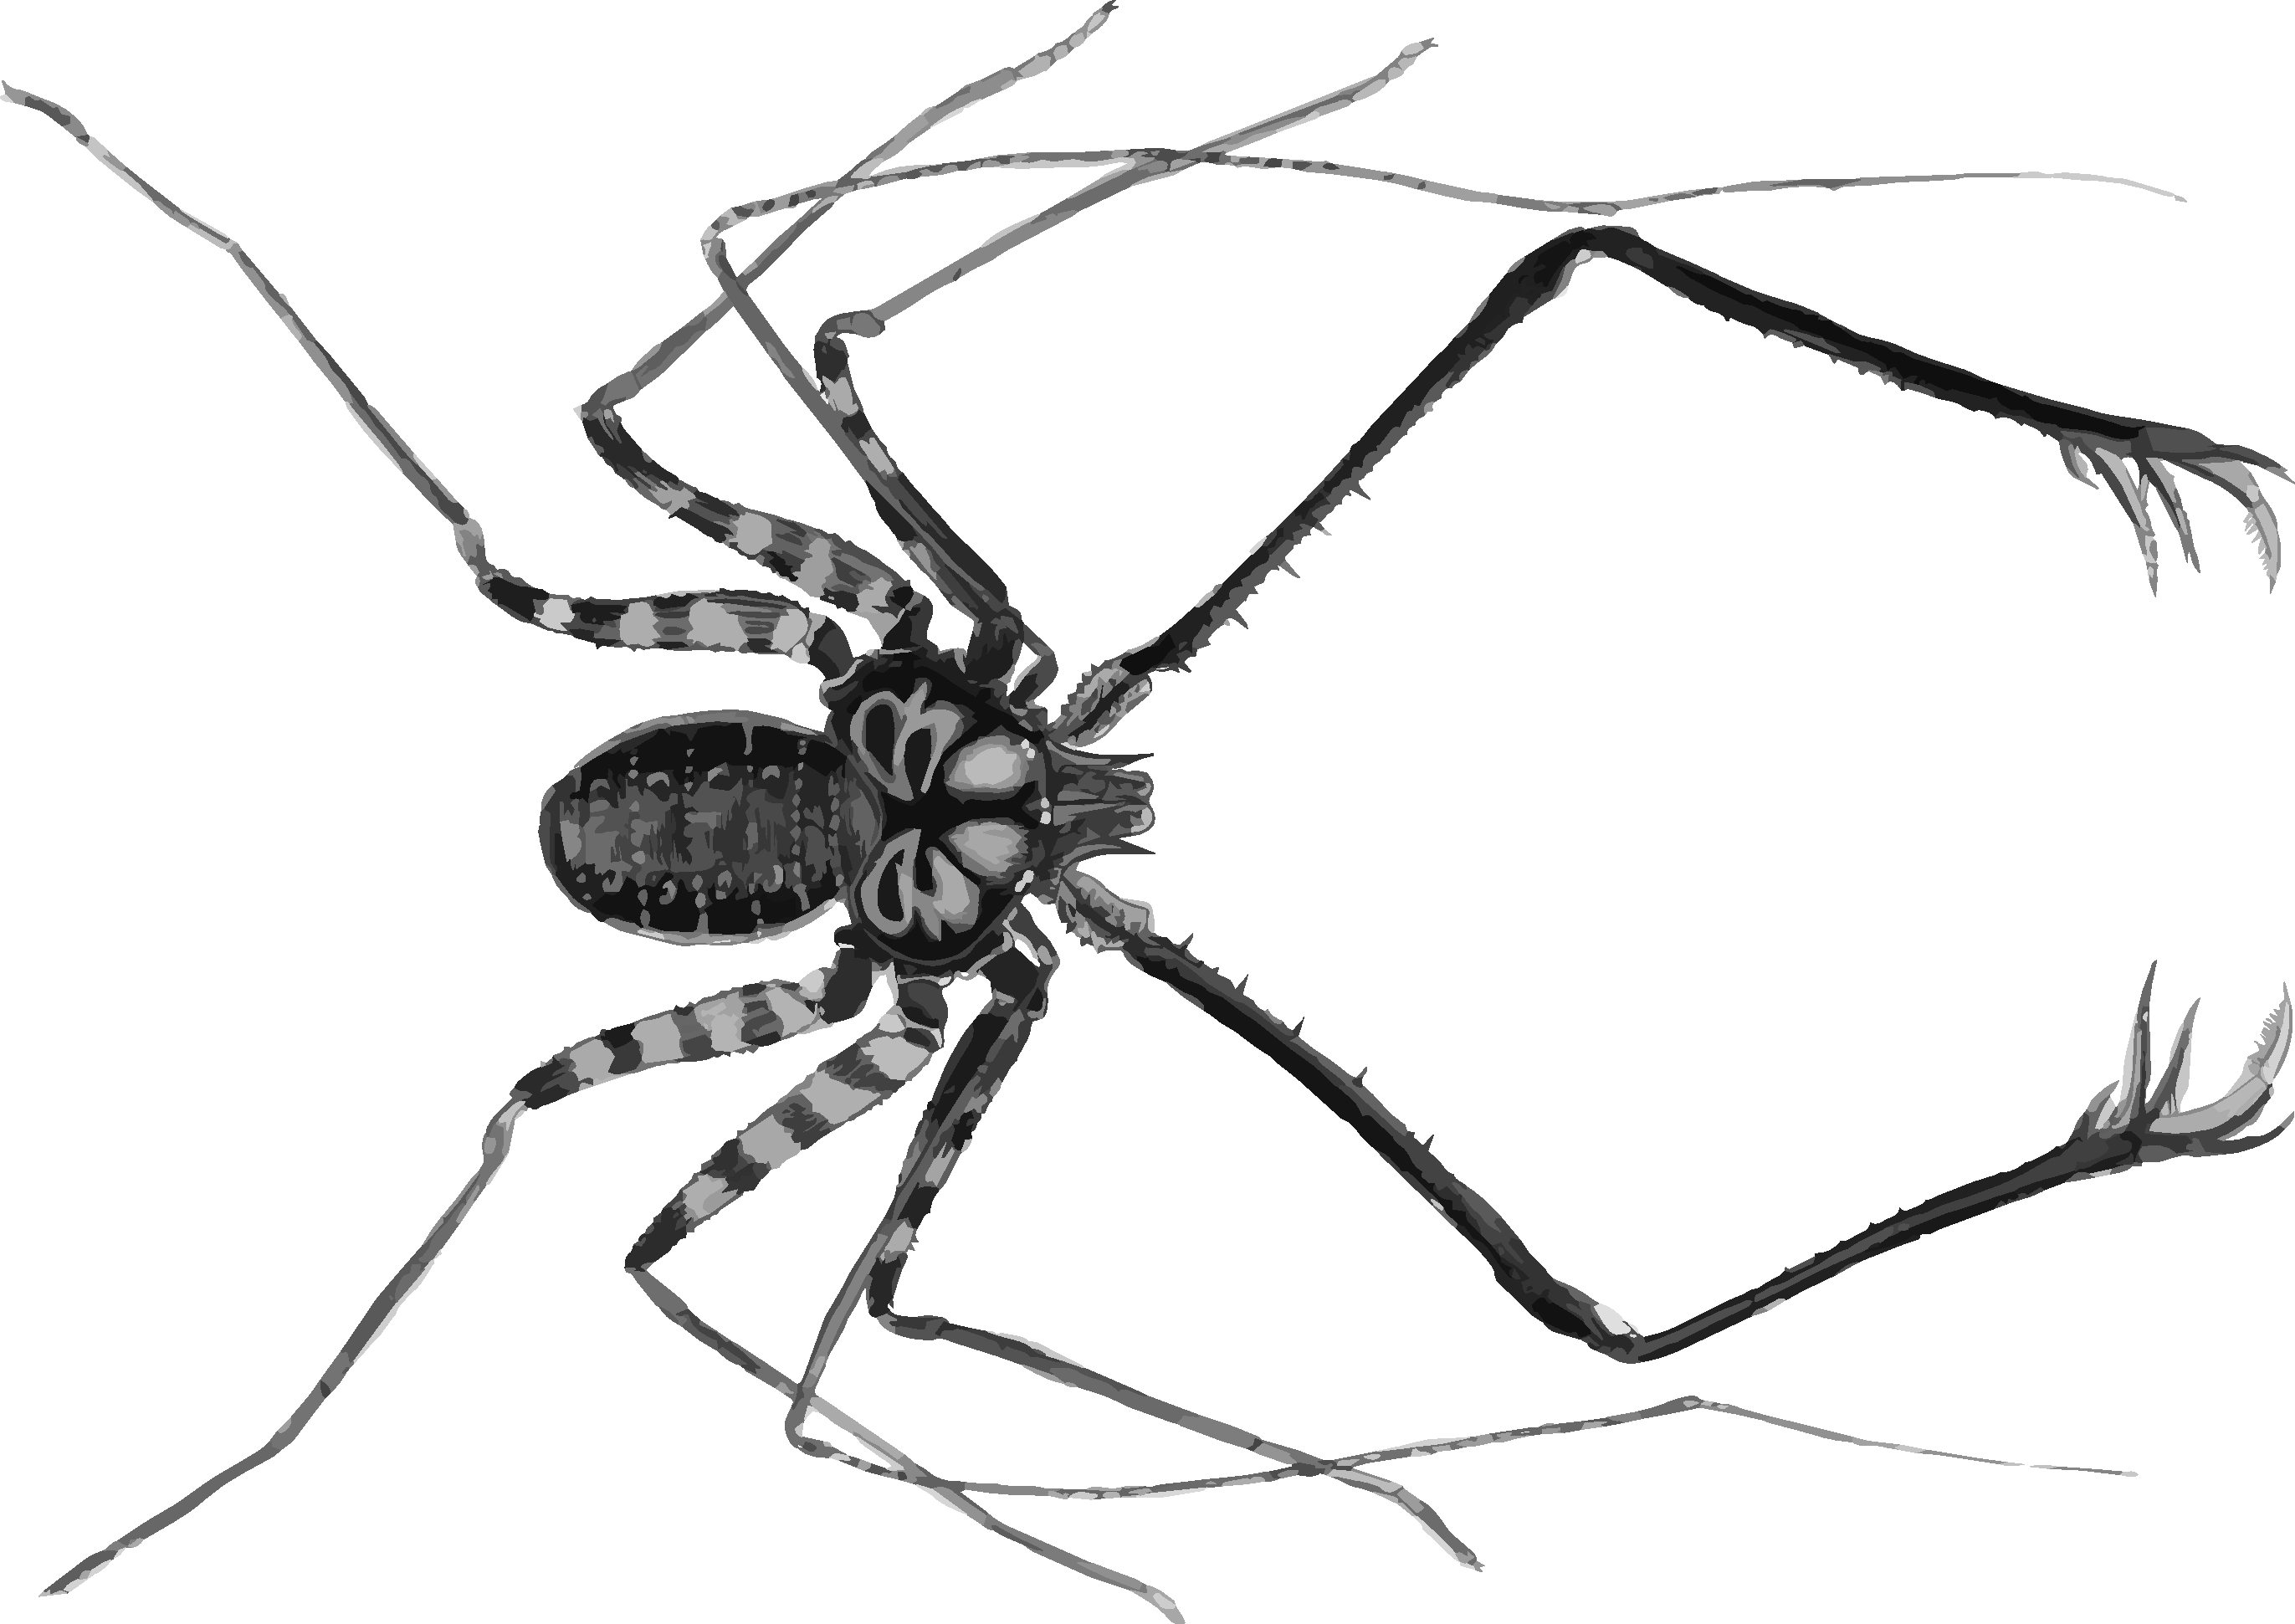
\includegraphics[width=0.55\textwidth]{nonhexapod/amblypygi}
  \caption{Amblypygi \citep[][plate CCCXXXVI]{bhlitem55834arach}}
  \label{fig:ambly1}
\end{figure}

\subsubsection*{Symphyla (symphylans)}\index{Symphyla}
Which major group does it belong in and why? What diagnostic characters separate it from the taxa above? What do these arthropods eat, and how do they live?\vspace{3mm}

\begin{figure}[ht!]
  \centering
    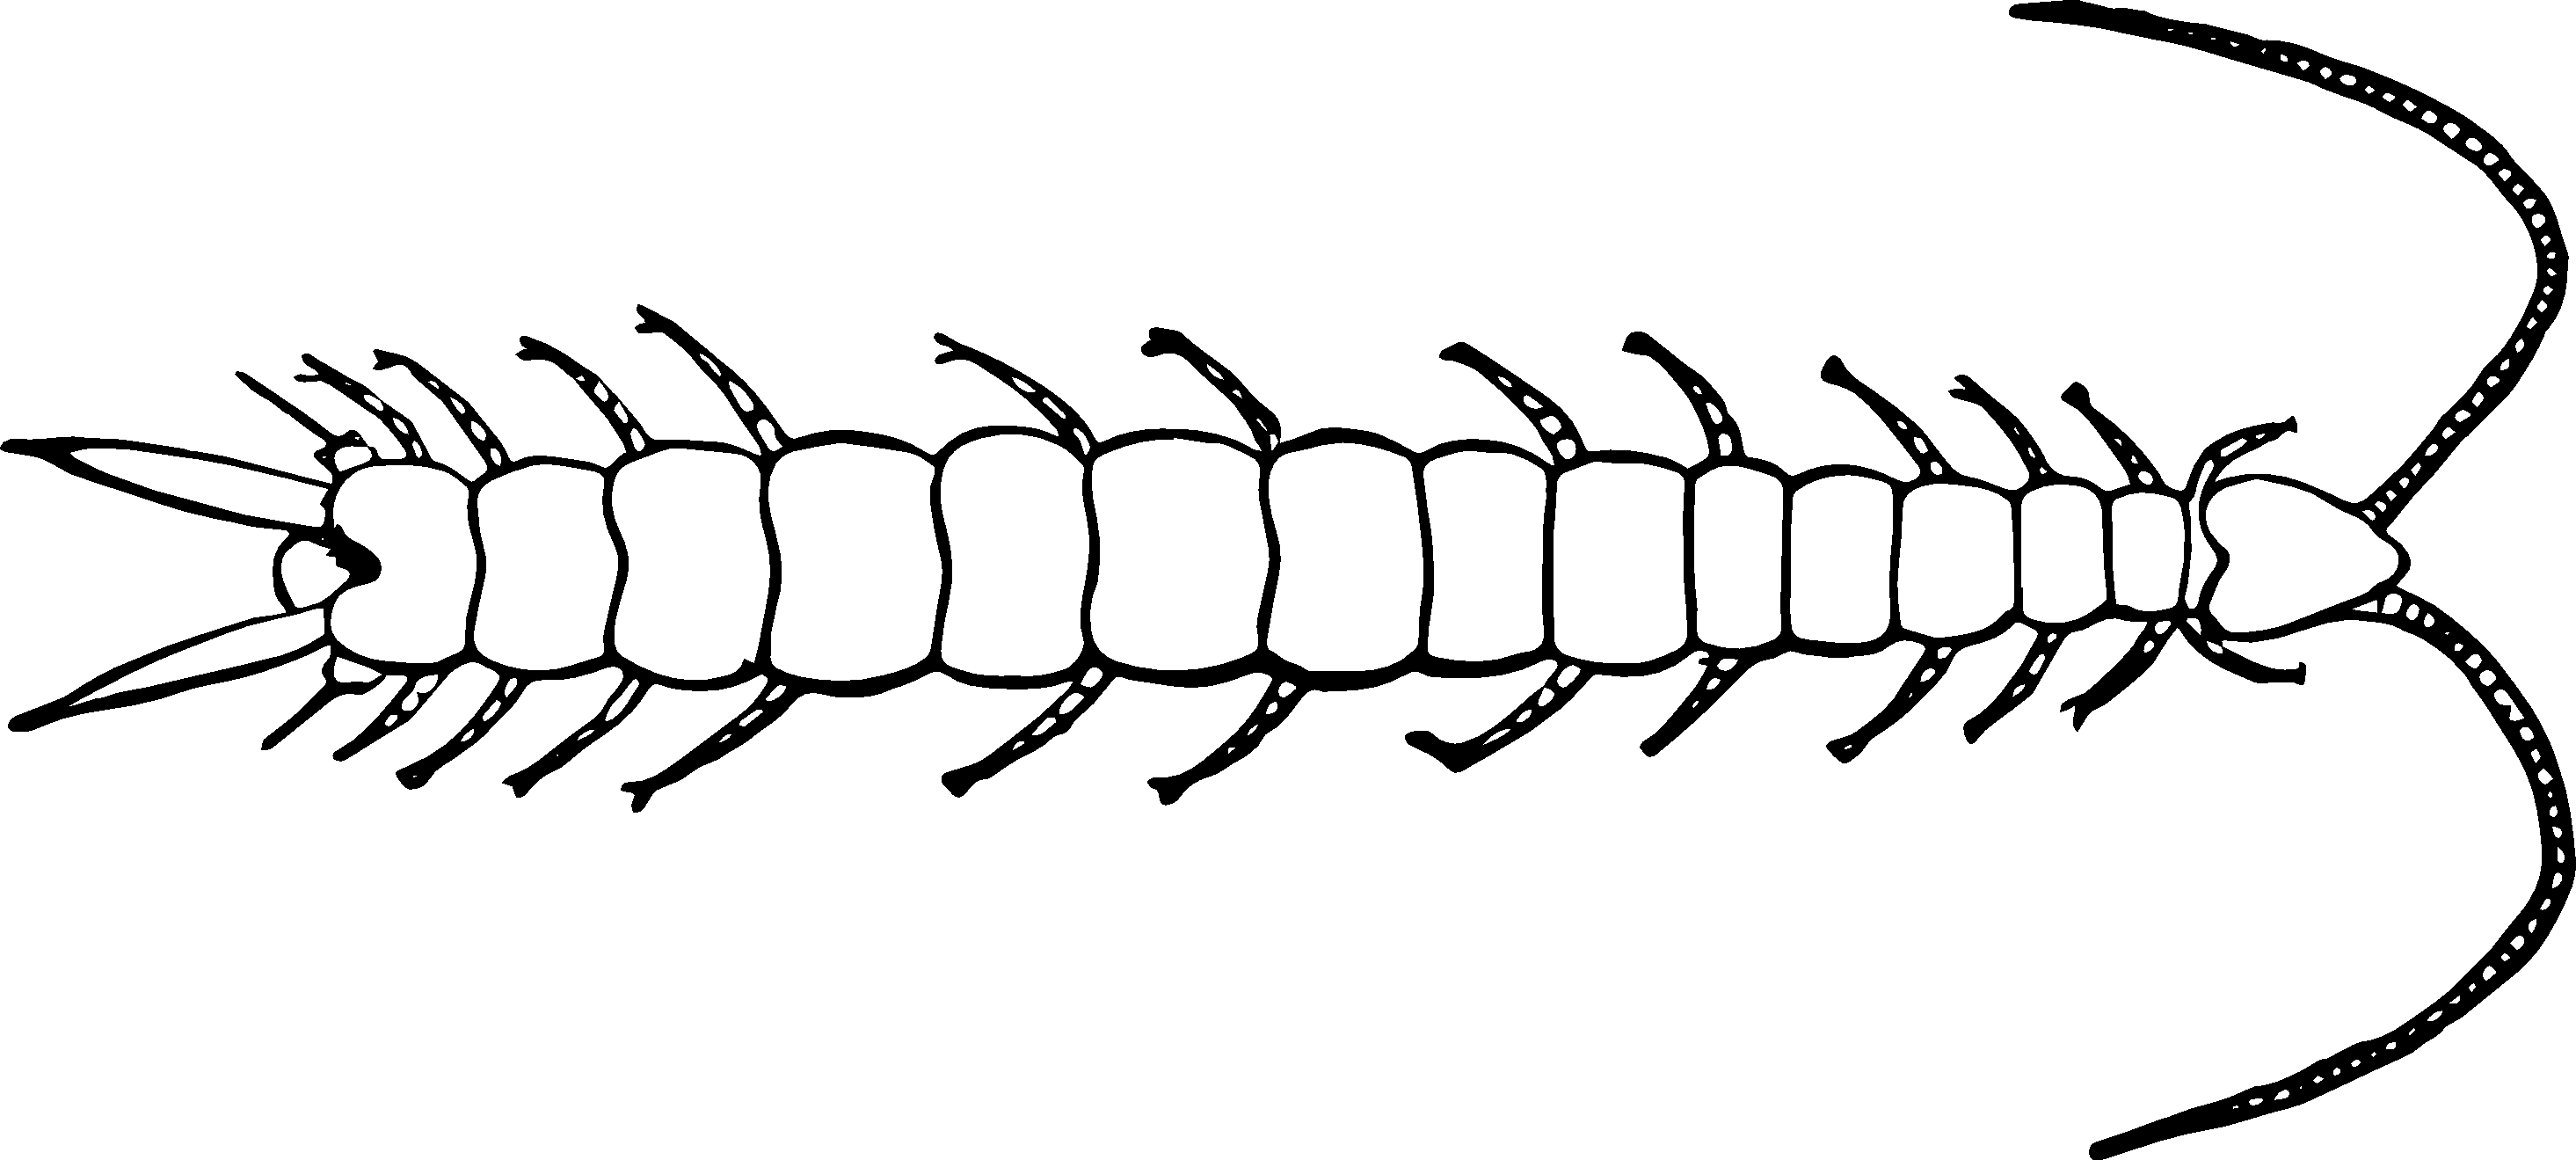
\includegraphics[width=0.55\textwidth]{nonhexapod/symphyla}
  \caption{Symphyla \citep[][Fig. 14B]{bhlitem16837entom}}
  \label{fig:symphyla}
\end{figure}

\section*{Test yourself}

\noindent{}Can you draw a phylogeny showing the relationships between Onychophora, Chelicerata, Myriapoda, and Pancrustacea (including Hexapoda)? Which node is the common ancestor of Arthropoda? \citep[Hint: see][]{Dunlop2013}\vspace{3mm}

\noindent{}Why are some of these taxa \textit{orders of magnitude} more diverse than others? For example, Araneae has at least 50,000 named species, whereas Amblypygi has merely 150 or so species. Diplopoda is comprised of \textit{thousands} of species, whereas Symphyla has merely 250 or so.

\clearpage
\thispagestyle{empty}
